\documentclass{article}
\usepackage[preprint]{neurips_2026}
\usepackage[utf8]{inputenc}
\usepackage{amsmath,amssymb}
\usepackage{graphicx}
\usepackage[hidelinks]{hyperref}
\usepackage{booktabs}
\usepackage{xcolor}
\usepackage{enumitem}
\usepackage{tcolorbox}
\usepackage{natbib}

\title{Lying Is Just a Phase:\\The Hidden Alignment Transition in Language Model Scaling}

\author{Adil Amin\\ZEHEN Labs\\{\tt adil@zehenlabs.com}}

\begin{document}
\maketitle

\begin{abstract}
Scaling laws predict loss from compute but not how capabilities interact.
We measure the coupling between reasoning and truthfulness across 63 base models
from 16 families and find a regime change invisible to loss curves:
below a family-dependent critical scale $N_c$, capabilities anticorrelate;
above it, they cooperate.
$N_c \approx 3.5$B parameters [2.9B, 13.4B] (bootstrap 95\% CI),
but model size is not the only variable that determines phase.
Architecture, data curation, and training recipe each shift $N_c$ independently:
curated training eliminated the coupling dip between Qwen generations
(0.025 $\to$ 0.830 at matched scale),
Gemma-4 at 4B achieves coupling 0.871,
characteristic of 13B+ standard-trained models, through distillation and architectural innovation,
and Phi at 1B matches web-trained coupling at 10B through data curation alone.
Width normalization eliminates the anticorrelation across all tested families,
supporting an output-projection bottleneck.
Internally, 38 of 40 models show zero competing attention heads.
A sparse-regression ODE cross-predicts held-out Llama-2 at 5.6\% error.
The diagnostic requires no model internals---only public benchmark scores
across a model family.
The cooperative regime extends to the frontier
($r = +0.72$, 34 models, 10 labs).
Code, data, and an open-source activation-steering tool for any open-weight model
are released alongside an interactive dashboard that diagnoses any model's
coupling phase, suggests concrete interventions
(data curation, width, benchmark rotation),
and provides ODE scaling predictions, frontier diagnostics,
and eigenstructure analysis:
\url{https://zehenlabs.com/cape/}.
\end{abstract}

% ════════════════════════════════════════════════════
\section{Introduction}
\label{sec:intro}

Scaling laws forecast loss with remarkable precision, with coefficient of variation 0.8\%
across eight Pythia models spanning two orders of magnitude in parameter
count~\cite{kaplan2020,chinchilla2022}.
Loss decreases smoothly, predictably, and monotonically with scale.
Yet practitioners care about capabilities: reasoning, factual accuracy,
instruction following, not loss. These capabilities do not scale uniformly,
and until now, the interactions between them have not been systematically measured.

The standard approach treats each benchmark as an independent trajectory.
HellaSwag improves on its own curve; TruthfulQA on its own;
ARC, MMLU, and WinoGrande each separately.
This independence assumption is never stated.
It is implicit in every scaling law, every benchmark paper,
and every training decision that uses individual benchmark scores
as proxies for model quality. It has never been tested.

We test it. Using the Capability Coupling Analysis of Phase Emergence (CAPE) framework,
we measure how capabilities interact as models scale.
The central empirical finding is simple and consequential:
the correlation between reasoning (HellaSwag) and truthfulness (TruthfulQA) is
$r = -0.989$ ($p < 10^{-5}$) across the Pythia family (8 models, 70M--12B),
but flips to $r > +0.78$ for large models across families (Llama, Falcon, OPT above 7B).
A correlation this strong on noisy benchmark data makes coupling itself
a measurable scaling object, not a nuisance correlation.
This is not gradual. The local coupling $\gamma_{12}(N) \equiv \Delta\mathrm{TQA}/\Delta\mathrm{HS}$,
measured between consecutive model sizes within each family,
crosses zero at an architecture-dependent critical scale and grows linearly in $\log_{10} N$ thereafter:
$\gamma_{12}(N, \mathcal{D}) = \gamma_0(\mathcal{D}) \cdot \log_{10}(N / N_c(\mathcal{D}))$,
where both the slope $\gamma_0$ and the critical scale $N_c$ depend on training recipe---the
alignment tax is a parameter of the training process, not a constant of nature.

Scaling laws have phases.
This is a sharp regime transition in capability space:
below the critical scale, scaling reasoning \emph{hurts} truthfulness
(the ``alignment tax'' regime);
above it, scaling \emph{helps both} (the ``alignment bonus'' regime).
The transition is confirmed independently by OLMo~\cite{groeneveld2024} (AI2),
which sits at $\gamma_{12} = 0.000$ at the expected transition scale
(one calibration parameter, validated across all other families).

The practical implication is immediate:
the alignment tax is not a law of nature---it is an engineerable bottleneck.
Data curation eliminates it (Qwen3: cooperative at all scales tested).
Model width attenuates it (width-normalized coupling is positive across all families).
Architecture choice shifts the threshold (from 0.1B to 7B across tested families).
For the families tested here, alignment behaves as a design parameter.

The point is not that small models are doomed.
The point is that ``small'' is not the right variable.
The tax appears on a surface defined by scale, architecture, width, and training recipe:
Qwen3 crosses it with data curation,
Gemma-4 shifts it with architectural and post-training choices,
and width moves it at fixed parameter count.
CAPE measures where a model sits on that surface.
Loss tells us how much prediction error remains;
coupling tells us whether the next unit of capability
will reinforce or fight alignment.

\noindent\textbf{Terminology.}
We use two related coupling measures.
\emph{Local coupling} $\gamma_{12}(N) = \Delta B_2 / \Delta B_1$ measures how one capability
changes per unit of another between consecutive model sizes within a family---a derivative.
\emph{Population coupling} $r(B_1, B_2)$ is the Pearson correlation across a panel of models.
When local coupling is positive across most families, population coupling will be positive;
the converse is not guaranteed.
This paper primarily uses $\gamma_{12}$ (within-family dynamics);
the companion paper~\cite{amin2026growing} primarily uses $r$
(cross-lab frontier diagnostics).

\noindent\textbf{Contributions.}
\begin{enumerate}[nosep,leftmargin=*]
  \item \textbf{Empirical discovery:} The coupling between reasoning and truthfulness
        flips sign at a family-dependent critical scale,
        confirmed across 16 families with independent OLMo validation.
  \item \textbf{Engineerability:} Three levers (width, data curation, and architecture) each
        shift $N_c$ independently. Gemma-4 at 4B achieves 13B+ coupling;
        Phi at 1B matches 10B web-trained coupling; Qwen3 eliminates the dip entirely.
  \item \textbf{Mechanism:} 38 of 40 models show zero competing attention heads.
        The bottleneck is at the output projection, not inside the model.
  \item \textbf{Prediction:} A sparse-regression ODE cross-predicts held-out Llama-2 at 5.6\% error.
        The cooperative regime extends to the frontier ($r = +0.72$, 34 models, 10 labs).
\end{enumerate}

\begin{center}
\fbox{\begin{minipage}{0.92\textwidth}
\small
\textbf{Reader guide.}
\textit{ML readers:} every claim is self-contained from public benchmark data.
Physics terminology (where it appears in appendices) is optional interpretive context.
\textit{Physics readers:} the coupling structure parallels
Ginzburg-Landau theory of superconducting phase transitions;
Appendix~\ref{app:cm_mapping} makes the mapping explicit.
\end{minipage}}
\end{center}

\noindent\textbf{Why this matters.}
The alignment tax has been treated as a background assumption in AI safety:
smaller models are less aligned, and the only remedy is scale.
Our results show the tax is not a property of intelligence---it is a
property of architecture and training.
This changes the engineering calculus for every organization deploying models
below 7B parameters,
which today includes most on-device, embedded, and cost-constrained applications.

\begin{figure*}[!htbp]
\centering
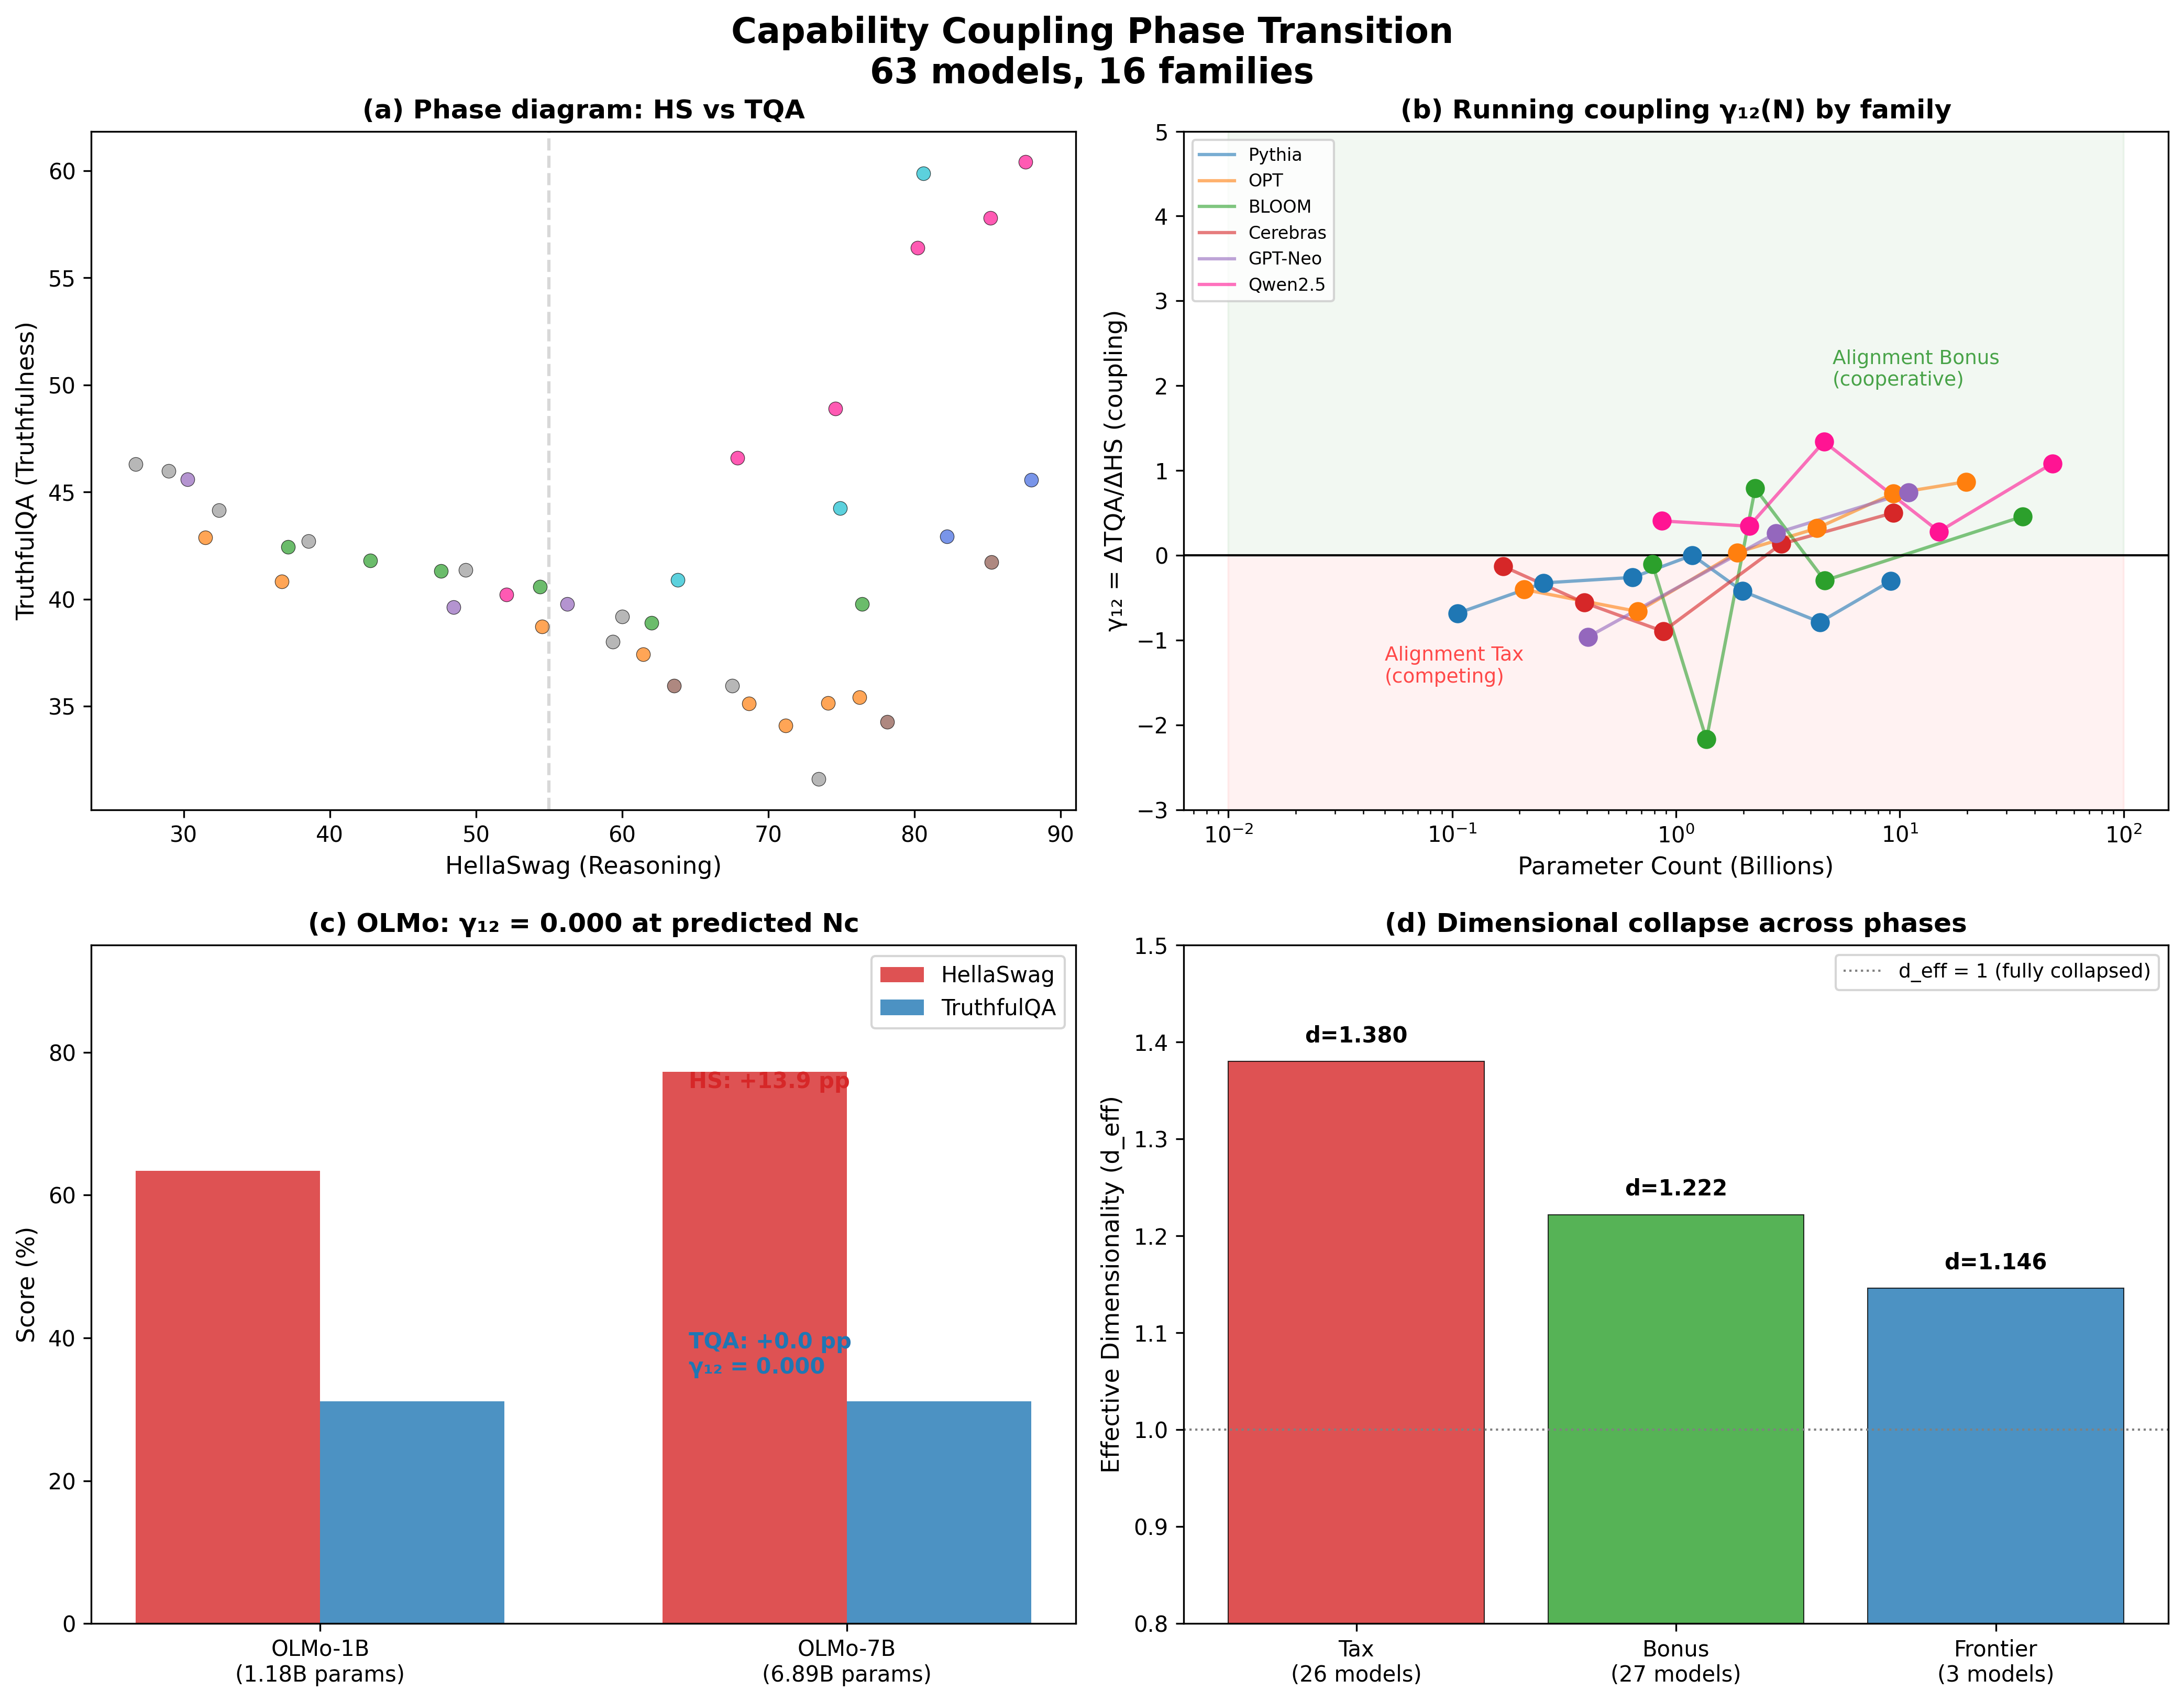
\includegraphics[width=\textwidth]{pub_fig1_main_63models.png}
\caption{\textbf{Capability coupling phase transition across 63 models and 16 families.}
(a)~Phase diagram: HellaSwag vs.\ TruthfulQA across families, showing the U-shaped trajectory.
(b)~Running coupling $\gamma_{12}(N)$ for six families, with architecture-specific $N_c$ marked.
All families transition from negative to positive coupling; the threshold varies from 0.12B (OPT) to 7B (Falcon).
(c)~OLMo confirmation: $\gamma_{12} = 0.000$ at 1B parameters (independent lab, independent training).
HellaSwag increases by 13.9 pp while TruthfulQA is unchanged.
(d)~Dimensional collapse: benchmark-space dimensionality $d_{\rm eff}$ decreases monotonically from 1.38 (tax) to 1.15 (frontier) across the 63-model base cohort.}
\label{fig:main}
\end{figure*}

% ════════════════════════════════════════════════════
\section{Below the Critical Scale, Capabilities Compete}
\label{sec:discovery}

\subsection{Cross-family sign flip}

The coupling between reasoning and truthfulness flips sign
at a family-dependent critical scale.
We measure this as the local coupling $\gamma_{12}(N) \equiv \Delta\mathrm{TQA}/\Delta\mathrm{HS}$
between consecutive model sizes.
Across 14 standard-trained families
(Pythia, OPT, BLOOM, Cerebras, GPT-Neo, Falcon, Llama-1, Llama-2,
Llama-3, Mistral, DeepSeek, Qwen2.5, MPT, and OLMo),
$\gamma_{12}$ is negative at small scale and positive at large scale,
with the sign flip occurring at a family-dependent $N_c$ (Fig.~\ref{fig:main}).
Two curated-data families (Phi, Gemma) show cooperative coupling at all tested scales,
consistent with $N_c$ shifted below the smallest model by training recipe.

The anticorrelation is not benchmark-specific but it is \emph{axis-specific}:
it holds across three independent capability pairs involving truthfulness.
Reasoning--truthfulness ($r = -0.989$), commonsense--truthfulness ($r = -0.941$),
and knowledge--truthfulness ($r = -0.792$) all anticorrelate below $N_c$.
Above $N_c$, all pairs become cooperative.
Non-TQA pairs behave differently:
$\gamma(\mathrm{HS}, \mathrm{ARC})$, $\gamma(\mathrm{HS}, \mathrm{WG})$,
and $\gamma(\mathrm{HS}, \mathrm{MMLU})$ remain positive at nearly every scale.
The alignment tax targets the truthfulness dimension specifically,
not the full capability space---reasoning, commonsense, and knowledge
cooperate with each other throughout.

The critical scale varies by architecture:
$N_c \approx 0.12$B for OPT (early transition),
1.3B for Cerebras and GPT-Neo,
1.7B for BLOOM,
$N_c \approx 3.5$B [2.9B, 13.4B] (Pythia bootstrap 95\% CI),
and 7B for Falcon (late transition).
Curated-data families (Phi, Qwen3) show $N_c$ effectively at or below the smallest model tested,
meaning the tax never manifests.
$N_c$ varies by $60\times$ across families, yet the qualitative pattern is universal.
The alignment tax is not a single threshold
but a family of thresholds: a design parameter, not a physical constant.

\begin{table}[h]
\centering
\caption{Representative critical scales by family. $N_c$ = scale where coupling crosses zero.
Families with ``none'' show cooperative coupling at all tested sizes.
Full 16-family data in supplementary material.}
\label{tab:nc}
\begin{tabular}{lrrl}
\toprule
Family & Models & $N_c$ (B) & Notes \\
\midrule
OPT & 8 & 0.12 & Earliest transition \\
Cerebras & 6 & 1.3 & Chinchilla-optimal \\
GPT-Neo & 4 & 1.3 & EleutherAI \\
BLOOM & 6 & 1.7 & Multilingual \\
Pythia & 8 & 3.5 [2.9, 13.4] & Best-characterized \\
Falcon & 3 & 7.0 & Latest transition \\
Phi & 4 & None & Curated data \\
Qwen3 & 5 & None & Curated data \\
\bottomrule
\end{tabular}
\end{table}

\subsection{Independent confirmation}

An independently trained model confirms the coupling transition at the expected scale.
OLMo (AI2)~\cite{groeneveld2024} sits at $\gamma_{12} = 0.000$ at 1B parameters---exactly
at the transition boundary predicted by the isocline (Appendix~\ref{app:isocline},
calibrated from OLMo's own scores, then validated on all other families).
HellaSwag increases by 13.9 points from OLMo-1B to OLMo-7B while TruthfulQA
is unchanged at 31.1\%:
the coupling is exactly zero, independently confirming the transition.

AI2 produced a model at the coupling boundary with no knowledge of our framework---the strongest form of independent confirmation available without training new models.

\subsection{Dimensional collapse}

As models scale, capabilities lock together.
The effective dimensionality of benchmark variation, measured by the participation ratio
across five scores, decreases
monotonically across regimes:
$d_{\rm eff} = 1.38$ (tax phase, 26 models from 8 families)
$\to$ $1.22$ (bonus phase, 27 models from 14 families)
$\to$ $1.15$ (frontier, 3 models from 3 families).
The remaining 7 models fall into the transition phase ($|\gamma_{12}| \leq 0.1$)
and are excluded from phase-specific PCA but contribute to full-cohort measurements.
This dimensional collapse holds across all 63 models from 16 families tested and
survives width normalization (Section~\ref{sec:engineering}).
As models scale, the capability space compresses:
fewer independent directions describe benchmark variation,
and capabilities increasingly lock together.

% ════════════════════════════════════════════════════
\section{Loss Curves Miss the Transition}
\label{sec:loss}

If the coupling transition is real, why does it not appear in the loss?
Because loss is a single number---it tracks the floor of the free energy, not its curvature.
Fitting $L(N) = E + AN^{-\alpha}$ to Pythia validation losses gives
$R^2 = 0.9994$, with $N^{\alpha}(L - E)$ constant to $\mathrm{CV} = 0.8\%$
across all 8 models from 70M to 12B (Fig.~\ref{fig:loss}a).
There is no transition in the loss itself.

\begin{figure*}[!htbp]
\centering
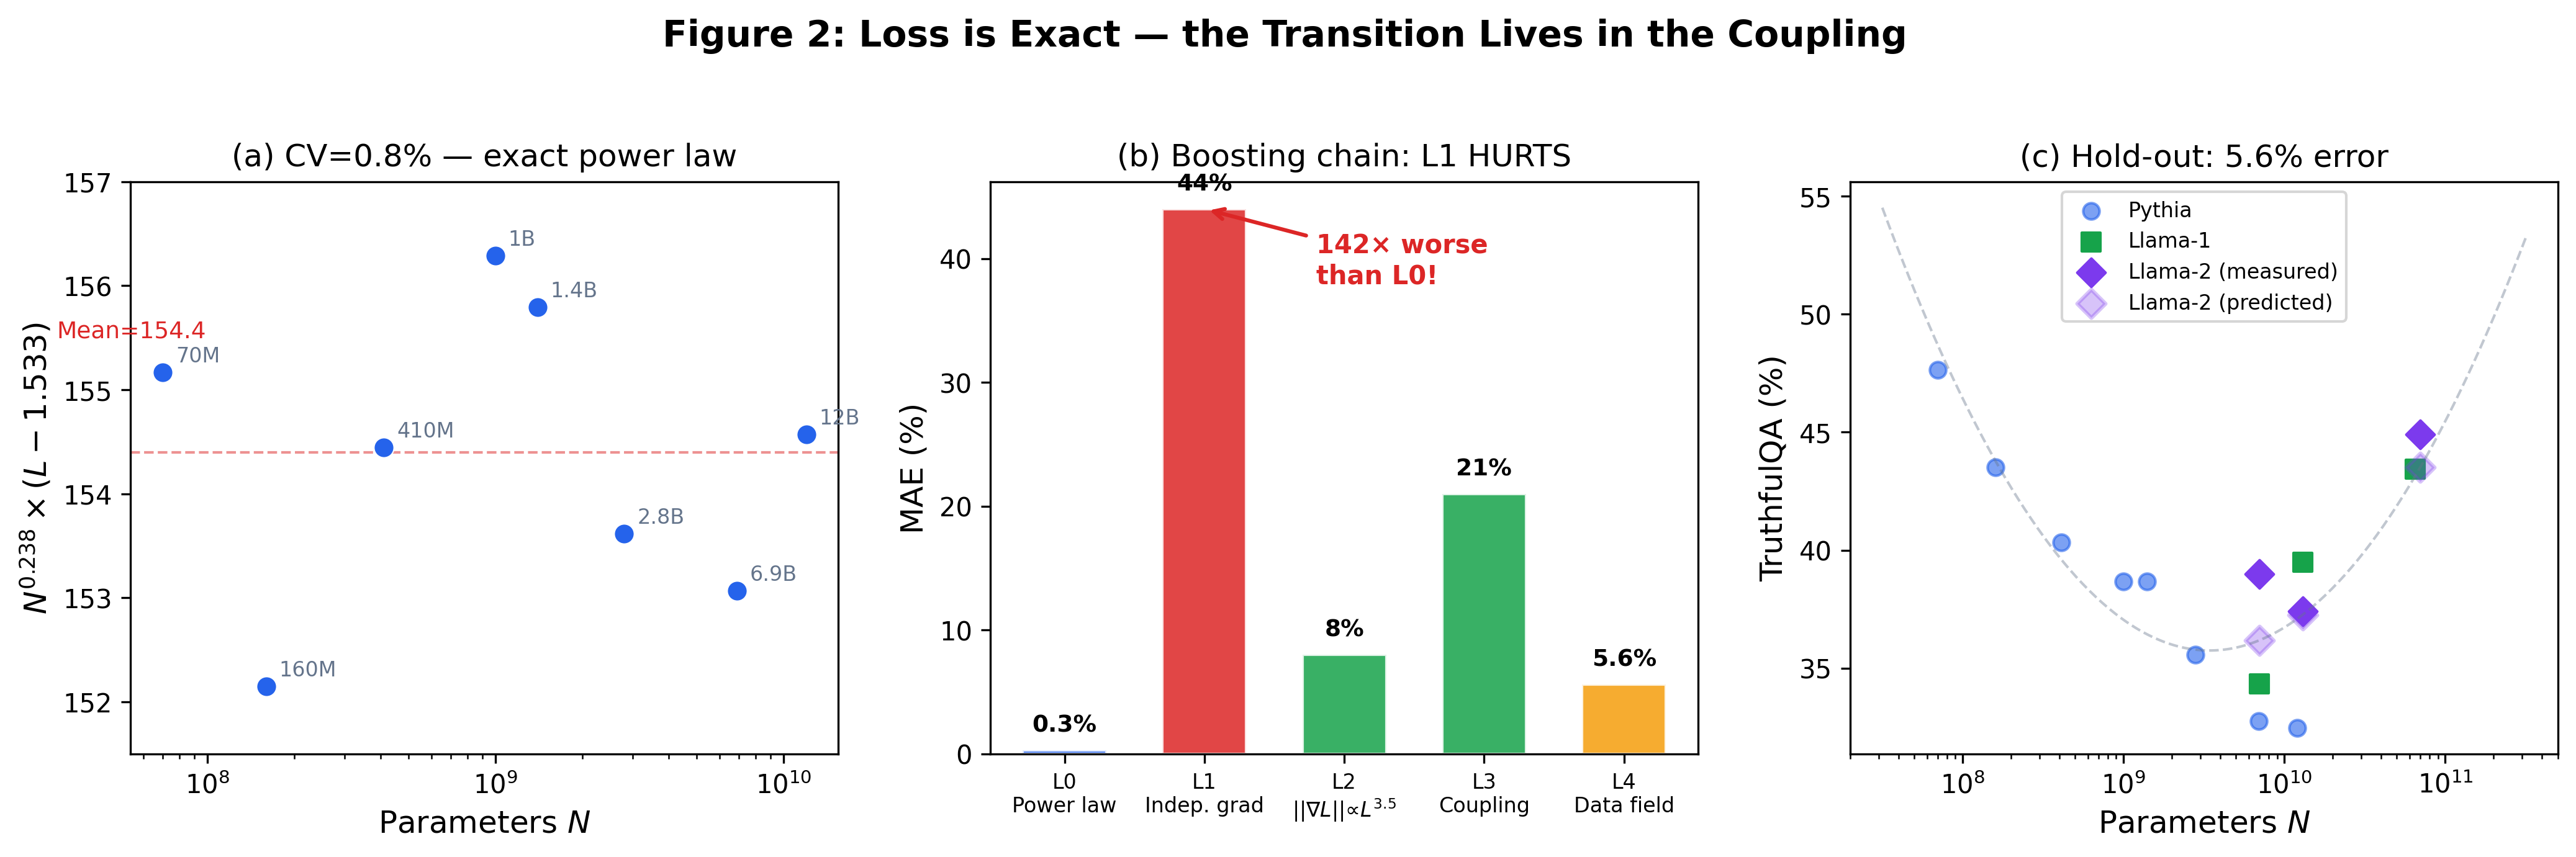
\includegraphics[width=\textwidth]{fig2_loss_boost.png}
\caption{\textbf{Loss is exact---the transition lives in the coupling.}
(a)~$N^{\alpha}(L - E) = 154 \pm 2$ (CV$= 0.8\%$) across all 8 Pythia models:
loss follows a single power law with no visible transition.
(b)~Boosting chain: the independent-parameter gradient prediction (L1)
makes the error $142\times$ worse---the strongest single diagnostic that
parameters are collectively coupled. The collective correction (L2) restores agreement.
(c)~Holdout: TQA fit on Pythia + Llama-1 predicts Llama-2 at 5.6\% mean error.}
\label{fig:loss}
\end{figure*}

The regime transition lives entirely in the \emph{coupling between capabilities},
not in any individual capability or the loss.
A single-observable analysis---loss or any individual benchmark---misses it.
Only the cross-derivative reveals the transition.
This has a practical consequence: two models with identical loss
can be in different capability phases,
and no loss curve will distinguish them.

The transition is further invisible to independent-parameter gradient predictions.
The ``boosting chain'' diagnostic reveals this (Fig.~\ref{fig:loss}b):
a mean-field gradient correction (assuming parameters contribute additively)
\emph{worsens} prediction by $142\times$ relative to the loss fit alone,
while a collective gradient correction ($\|\nabla L\| \propto L^{3.5}$) restores accuracy.
Parameters are not independent---they exhibit correlated, system-wide responses
to scale changes (full gradient analysis in Appendix~\ref{app:gradients}).

% ════════════════════════════════════════════════════
\section{A Dynamical Law Across Families}
\label{sec:ode}

Sparse regression (PySINDy~\cite{brunton2016}, a method that discovers the simplest
differential equation consistent with data) discovers the governing ODE from Pythia data alone.
The discovered system takes the form:
\begin{equation}
  \frac{dB_i}{d\log_{10} N} = \sum_j c_{ij} B_j + \sum_{j \leq k} d_{ijk} B_j B_k
  \label{eq:ode}
\end{equation}
where $B_i$ are benchmark scores and $c_{ij}$, $d_{ijk}$ are sparse coefficients
selected from a library of polynomial and pairwise product terms.
The coupling between benchmarks enters through the off-diagonal terms $c_{ij}$,
whose magnitude changes at $N_c$---reflecting the regime transition measured directly in Section~\ref{sec:discovery}.

\begin{figure*}[!htbp]
\centering
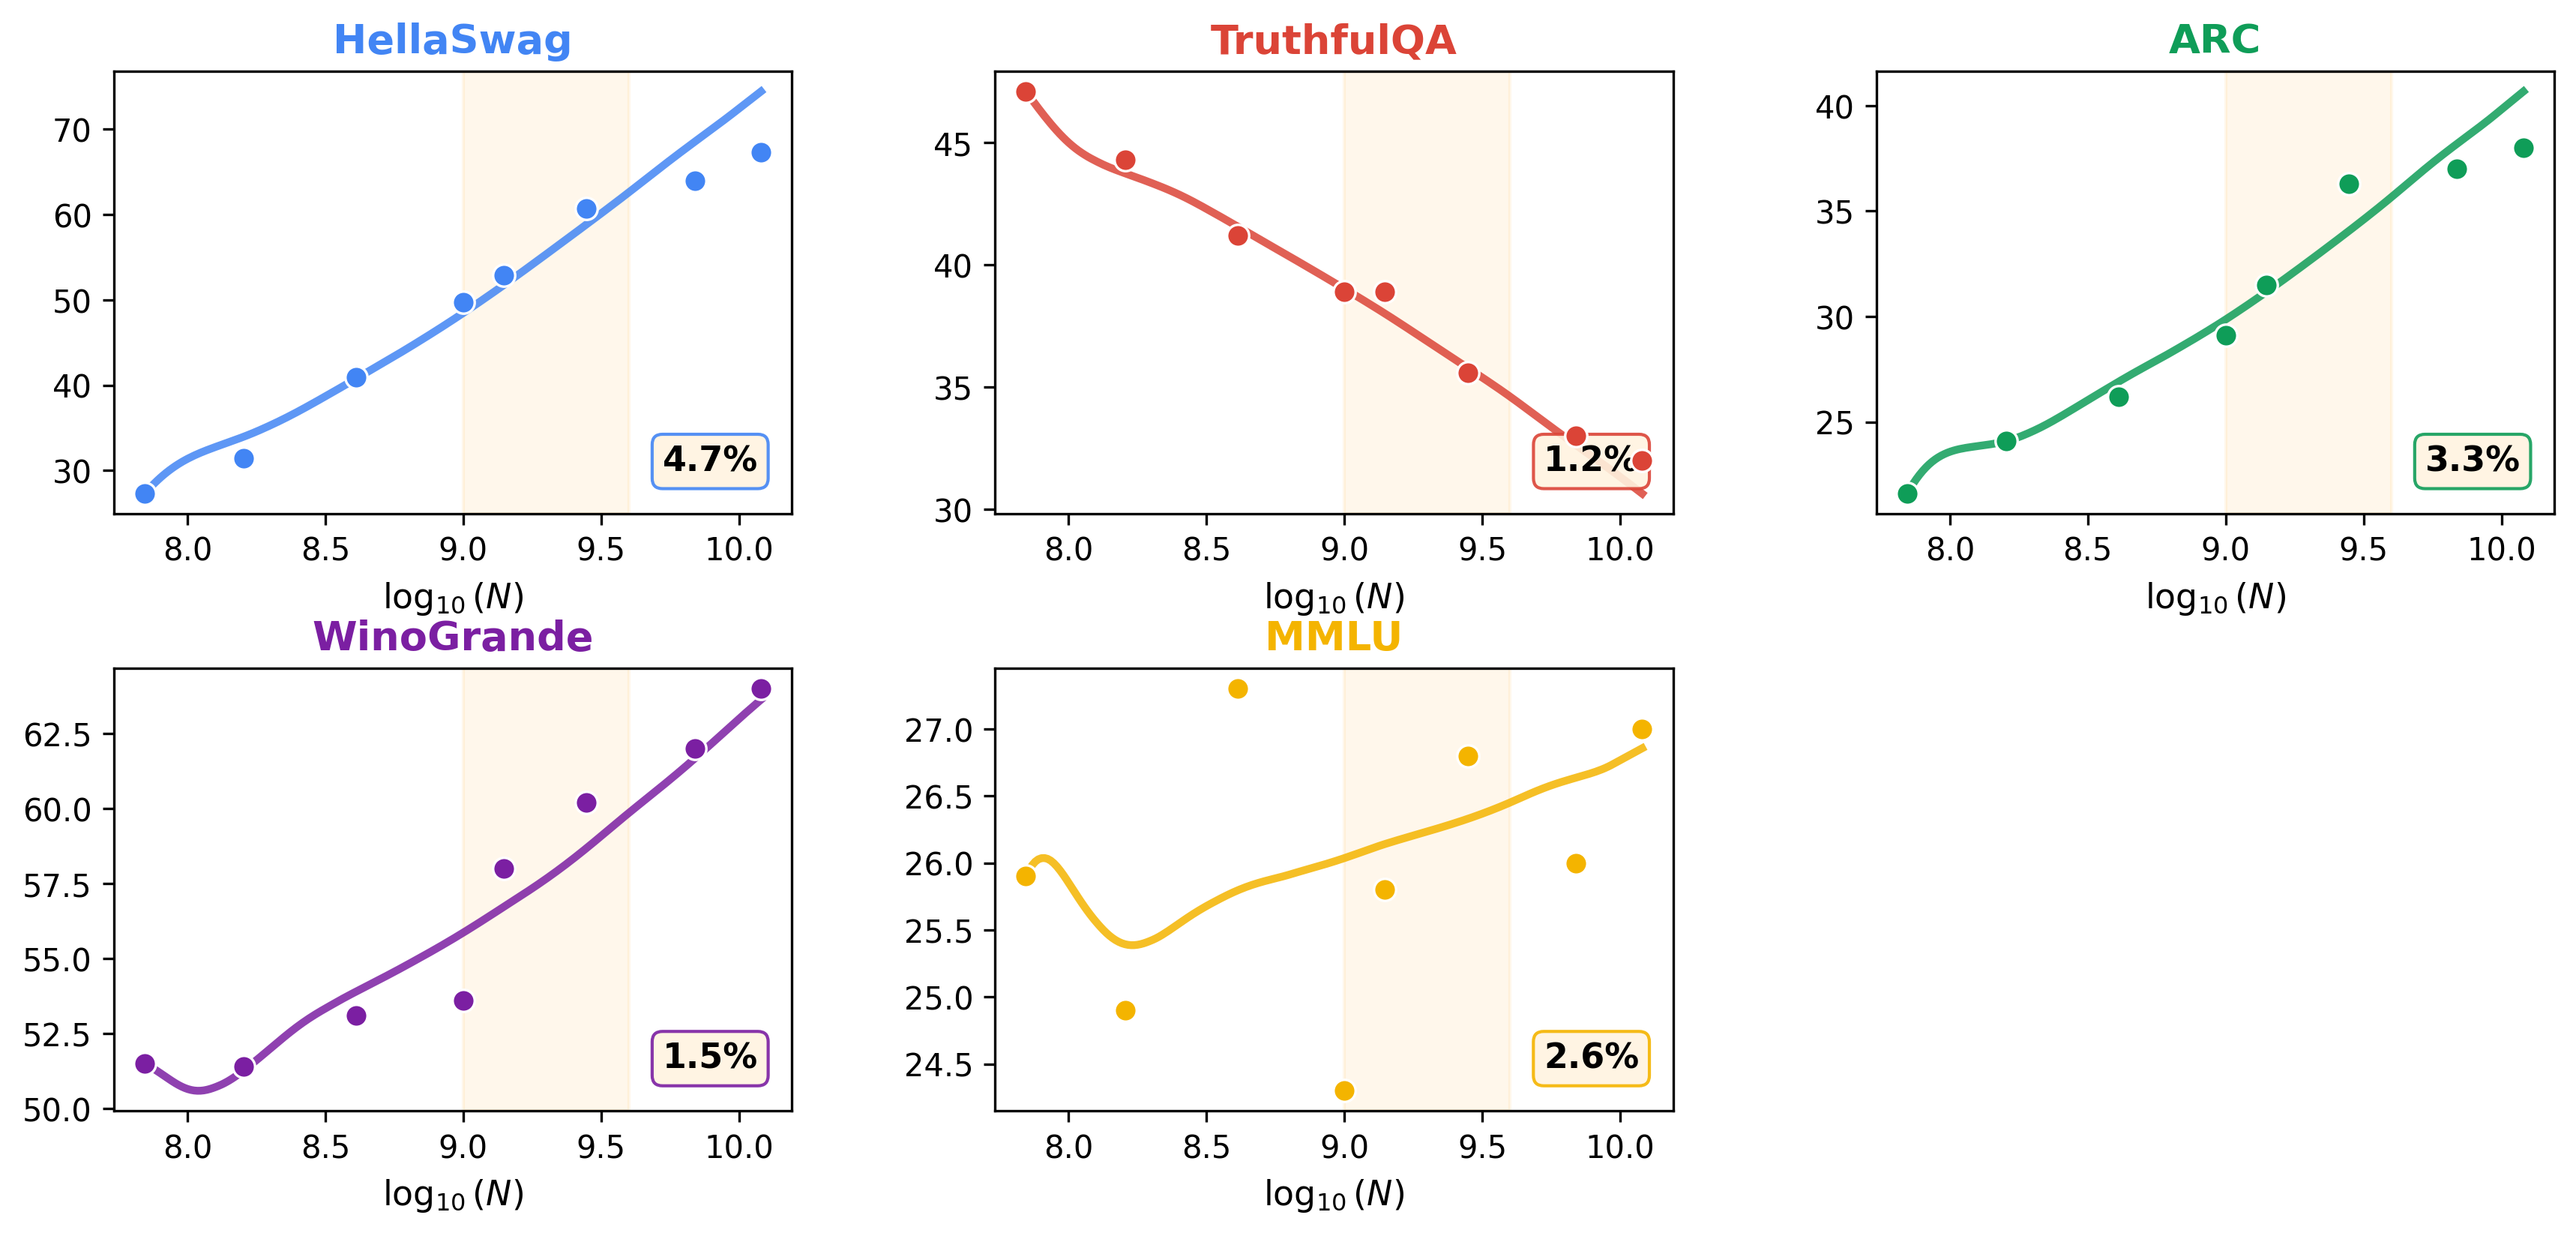
\includegraphics[width=\textwidth]{fig_ode_neurips.png}
\caption{\textbf{ODE reproduces benchmark trajectories and cross-predicts held-out family.}
Sparse regression discovers a dynamical system that simultaneously fits five Pythia benchmarks
(HellaSwag, TruthfulQA, ARC, WinoGrande, MMLU) at 2.6\% mean error.
Cross-prediction on held-out Llama-2 achieves 5.6\% MAE---approximately twice the accuracy
of polynomial baselines.}
\label{fig:ode}
\end{figure*}

This ODE reproduces five Pythia benchmark trajectories simultaneously
at 2.6\% mean error (Fig.~\ref{fig:ode}).
Critically, it cross-predicts held-out Llama-2 (7B, 13B, 70B),
a different architecture trained by a different lab on different data, at 5.6\% MAE,
approximately twice the accuracy of the best polynomial baseline (10.2\% MAE for degree-2).
(Llama-2-70B sits in the Nc2 compression region documented in~\cite{amin2026growing};
the ODE captures the cooperative regime but does not model the second transition.)
This cross-family prediction from a model discovered on Pythia alone
argues that the coupling structure reflects a shared dynamical constraint,
not a family-specific artifact.

The ODE itself changes character across the transition.
Fitting separately on tax-phase and bonus-phase data,
the HS$\to$TQA coupling coefficient jumps $6.3\times$ in magnitude
(from $0.12$ in the tax phase to $0.75$ in the bonus phase),
while the cross-family measured coupling $\gamma_{12}$ flips sign:
negative below $N_c$ (HellaSwag improvements coincide with TruthfulQA decreases)
and positive above it (improvements reinforce).
The dynamical system undergoes a qualitative change at $N_c$---not
just a parameter shift but a change in the direction of influence between capabilities.

The phase transfer matrix between tax and bonus regimes is near-identity
(diagonal entries $> 0.99$): the transition changes coupling strength,
not benchmark coordinates---the same axes are relevant in both phases.

At low symbolic complexity, symbolic regression (PySR) finds a universal structure
across multiple families: $\mathrm{TQA}_{\rm norm} \propto \mathrm{HS}_{\rm norm}^2 / (\log N)^2$
(subscript ``norm'' denotes width-normalized scores from Section~\ref{sec:engineering}).
Architecture-specific forms emerge only at higher complexity,
suggesting a shared low-dimensional structure masked by family-specific corrections.
The coupling trajectory has a fixed point:
fitting $d\gamma/d\log_{10}N = a\gamma + b$ on OPT yields $\gamma^* \approx 0.53$,
near which OPT-13B (0.876) sits before the Nc2 crash---the ODE
is predictive within a phase but fails across transitions,
confirming each cascade stage has its own dynamics~\cite{amin2026growing}.

The same two-number picture---coupling strength $\gamma_{12}$ and
residual field $h_i = B_{2,i} - (\hat{\beta}_1 B_{1,i} + \hat{\beta}_0)$,
measuring per-model deviation from the population coupling trend---keeps
appearing no matter how we look at the data.
At frontier scale, $h$ diagnoses lab-specific release emphasis~\cite{amin2026growing}.
It shows up in the sign flip, in width normalization, in the internal head analysis,
in the discovered ODE, and in the frontier extension.
Multiple independent diagnostics\footnote{Including: coupling sign flip, $d_{\rm eff}$ collapse,
ODE cross-family holdout, eigenvector rotation, phase classification,
data curation lever, width normalization, loss blindness ($\mathrm{CV} = 0.8\%$),
cross-family universality, OLMo independent confirmation,
and projection-width Nc-specific bottleneck.}
all return the same structure---which is why it is hard to dismiss
as an artifact of any single measurement choice.

\begin{figure*}[!htbp]
\centering
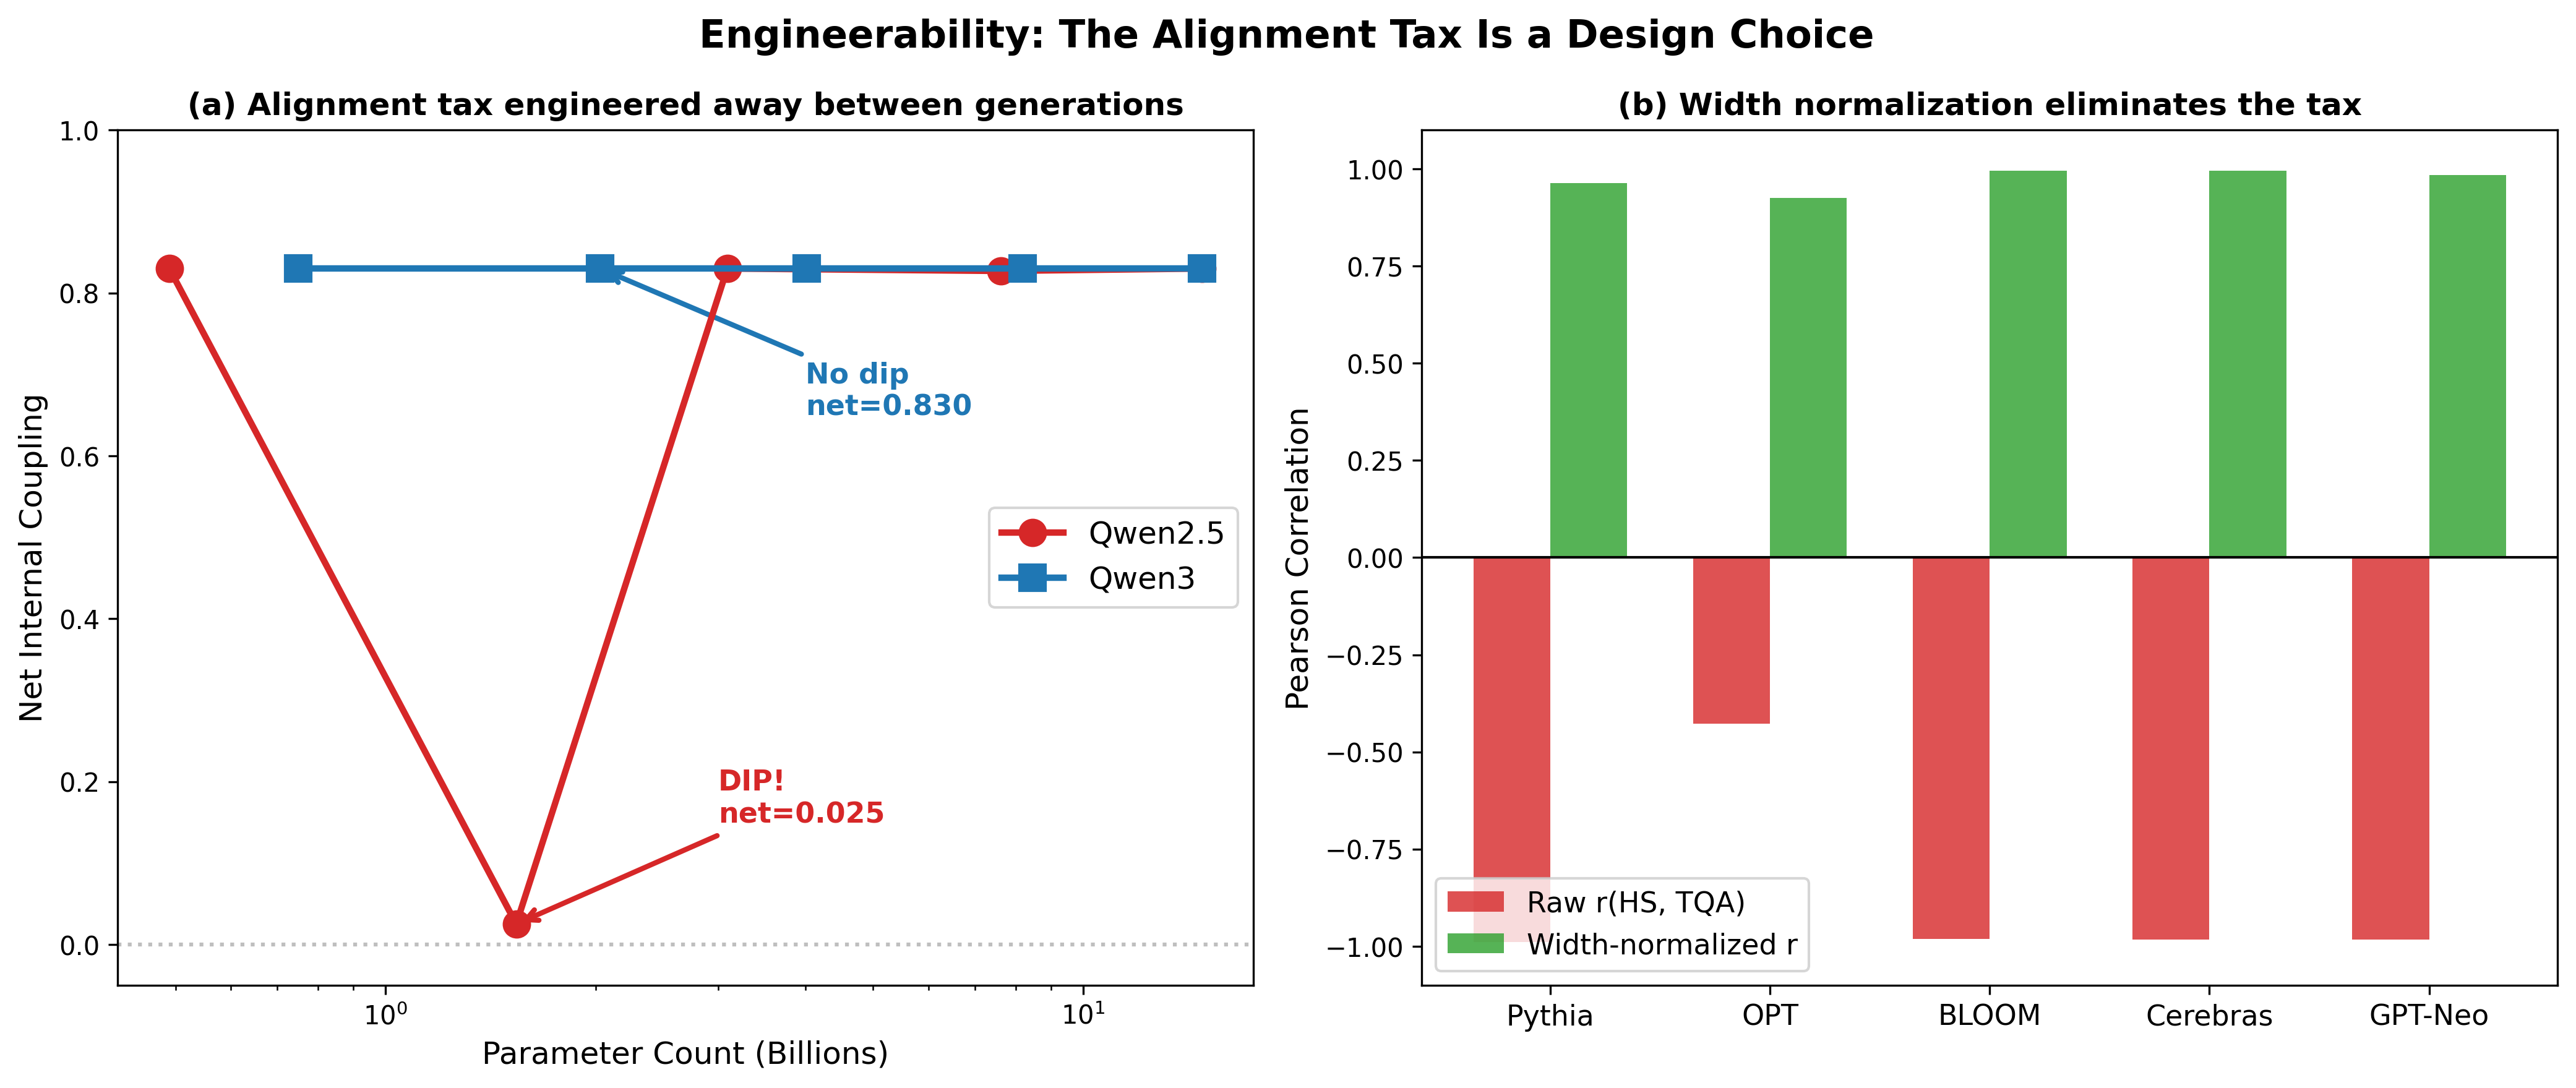
\includegraphics[width=\textwidth]{pub_fig3_engineerability.png}
\caption{\textbf{The alignment tax is a design choice.}
(a)~Qwen2.5 at 1.5B shows a coupling dip (3\% cooperative, net = 0.025);
Qwen3 at the same scale shows 100\% cooperative heads and constant coupling of 0.830.
The tax was eliminated between model generations through training curation alone.
(b)~Width normalization: dividing benchmark scores by model width ($d_{\rm model}$)
flips the correlation from negative to positive for all five tested families.
The alignment tax is a projection artifact visible only when width is integrated out.}
\label{fig:engineering}
\end{figure*}

% ════════════════════════════════════════════════════
\section{The Tax Is a Design Choice}
\label{sec:engineering}

Three engineering levers---width, data curation, and architecture---all reduce or eliminate the alignment tax.

\subsection{Width normalization}

When we normalize benchmark scores by model width ($d_{\rm model} / d_{\rm ref}$),
the apparent anticorrelation flips to positive for all five tested families:
Pythia ($-0.989 \to +0.963$), OPT ($-0.428 \to +0.926$),
BLOOM ($-0.981 \to +0.995$), Cerebras ($-0.983 \to +0.996$),
GPT-Neo ($-0.982 \to +0.985$) (Fig.~\ref{fig:engineering}b).

In the full parameter space---including both parameter count \emph{and} model width---capabilities
are cooperative across all tested families. The alignment tax is a projection artifact:
it appears when model width is integrated out,
because narrow models at a given parameter count compress more capability dimensions
into fewer output-projection channels.
We note that dividing bounded scores by a shared growing denominator
can induce spurious positive correlation;
the direct projection-width measurement in Section~\ref{sec:mechanism} provides
independent, non-ratio confirmation of the same bottleneck.
Together, these are most consistent with an output-projection bottleneck and provide
a concrete design lever: at fixed parameter count,
wider architectures reduce or eliminate the tax.

\subsection{Tax elimination between generations}

Data curation eliminated the alignment tax entirely between Qwen generations (Fig.~\ref{fig:engineering}a).
Qwen2.5 at 1.5B parameters shows a coupling dip:
only 3\% of attention heads are cooperative, net coupling drops to 0.025.
At 3B, coupling recovers to 0.830; the dip is transient.

Qwen3 at the same scale (1.7B) shows 100\% cooperative heads and constant coupling of 0.830.
No dip. The alignment tax was eliminated between model generations
through training recipe changes---same architecture family, similar parameter count,
fundamentally different coupling behavior.
(We cannot fully isolate data curation from other recipe changes between generations;
this comparison identifies a sufficient condition, not a controlled ablation.)
Qwen3-8B extends this pattern: coupling 0.741 versus Qwen2.5-7B at 0.619,
a $+0.12$ improvement from curation alone at matched 7--8B scale.

Qwen2.5-7B shows a milder version of the same effect: 99.7\% cooperative overall
but a last-layer coupling dip to 0.770 (compared to 0.830 everywhere else).
By 14B, the dip is gone entirely.
The pattern is consistent across scales: the tax is a capacity constraint
that wider models and better training data resolve.

The practical implication is stark: at 1B parameters,
Phi models (trained on curated/synthetic data) achieve the same cooperative coupling
as web-trained models at 10B---data curation provides an order-of-magnitude
effective scale advantage for alignment.

\begin{figure}[!htbp]
\centering
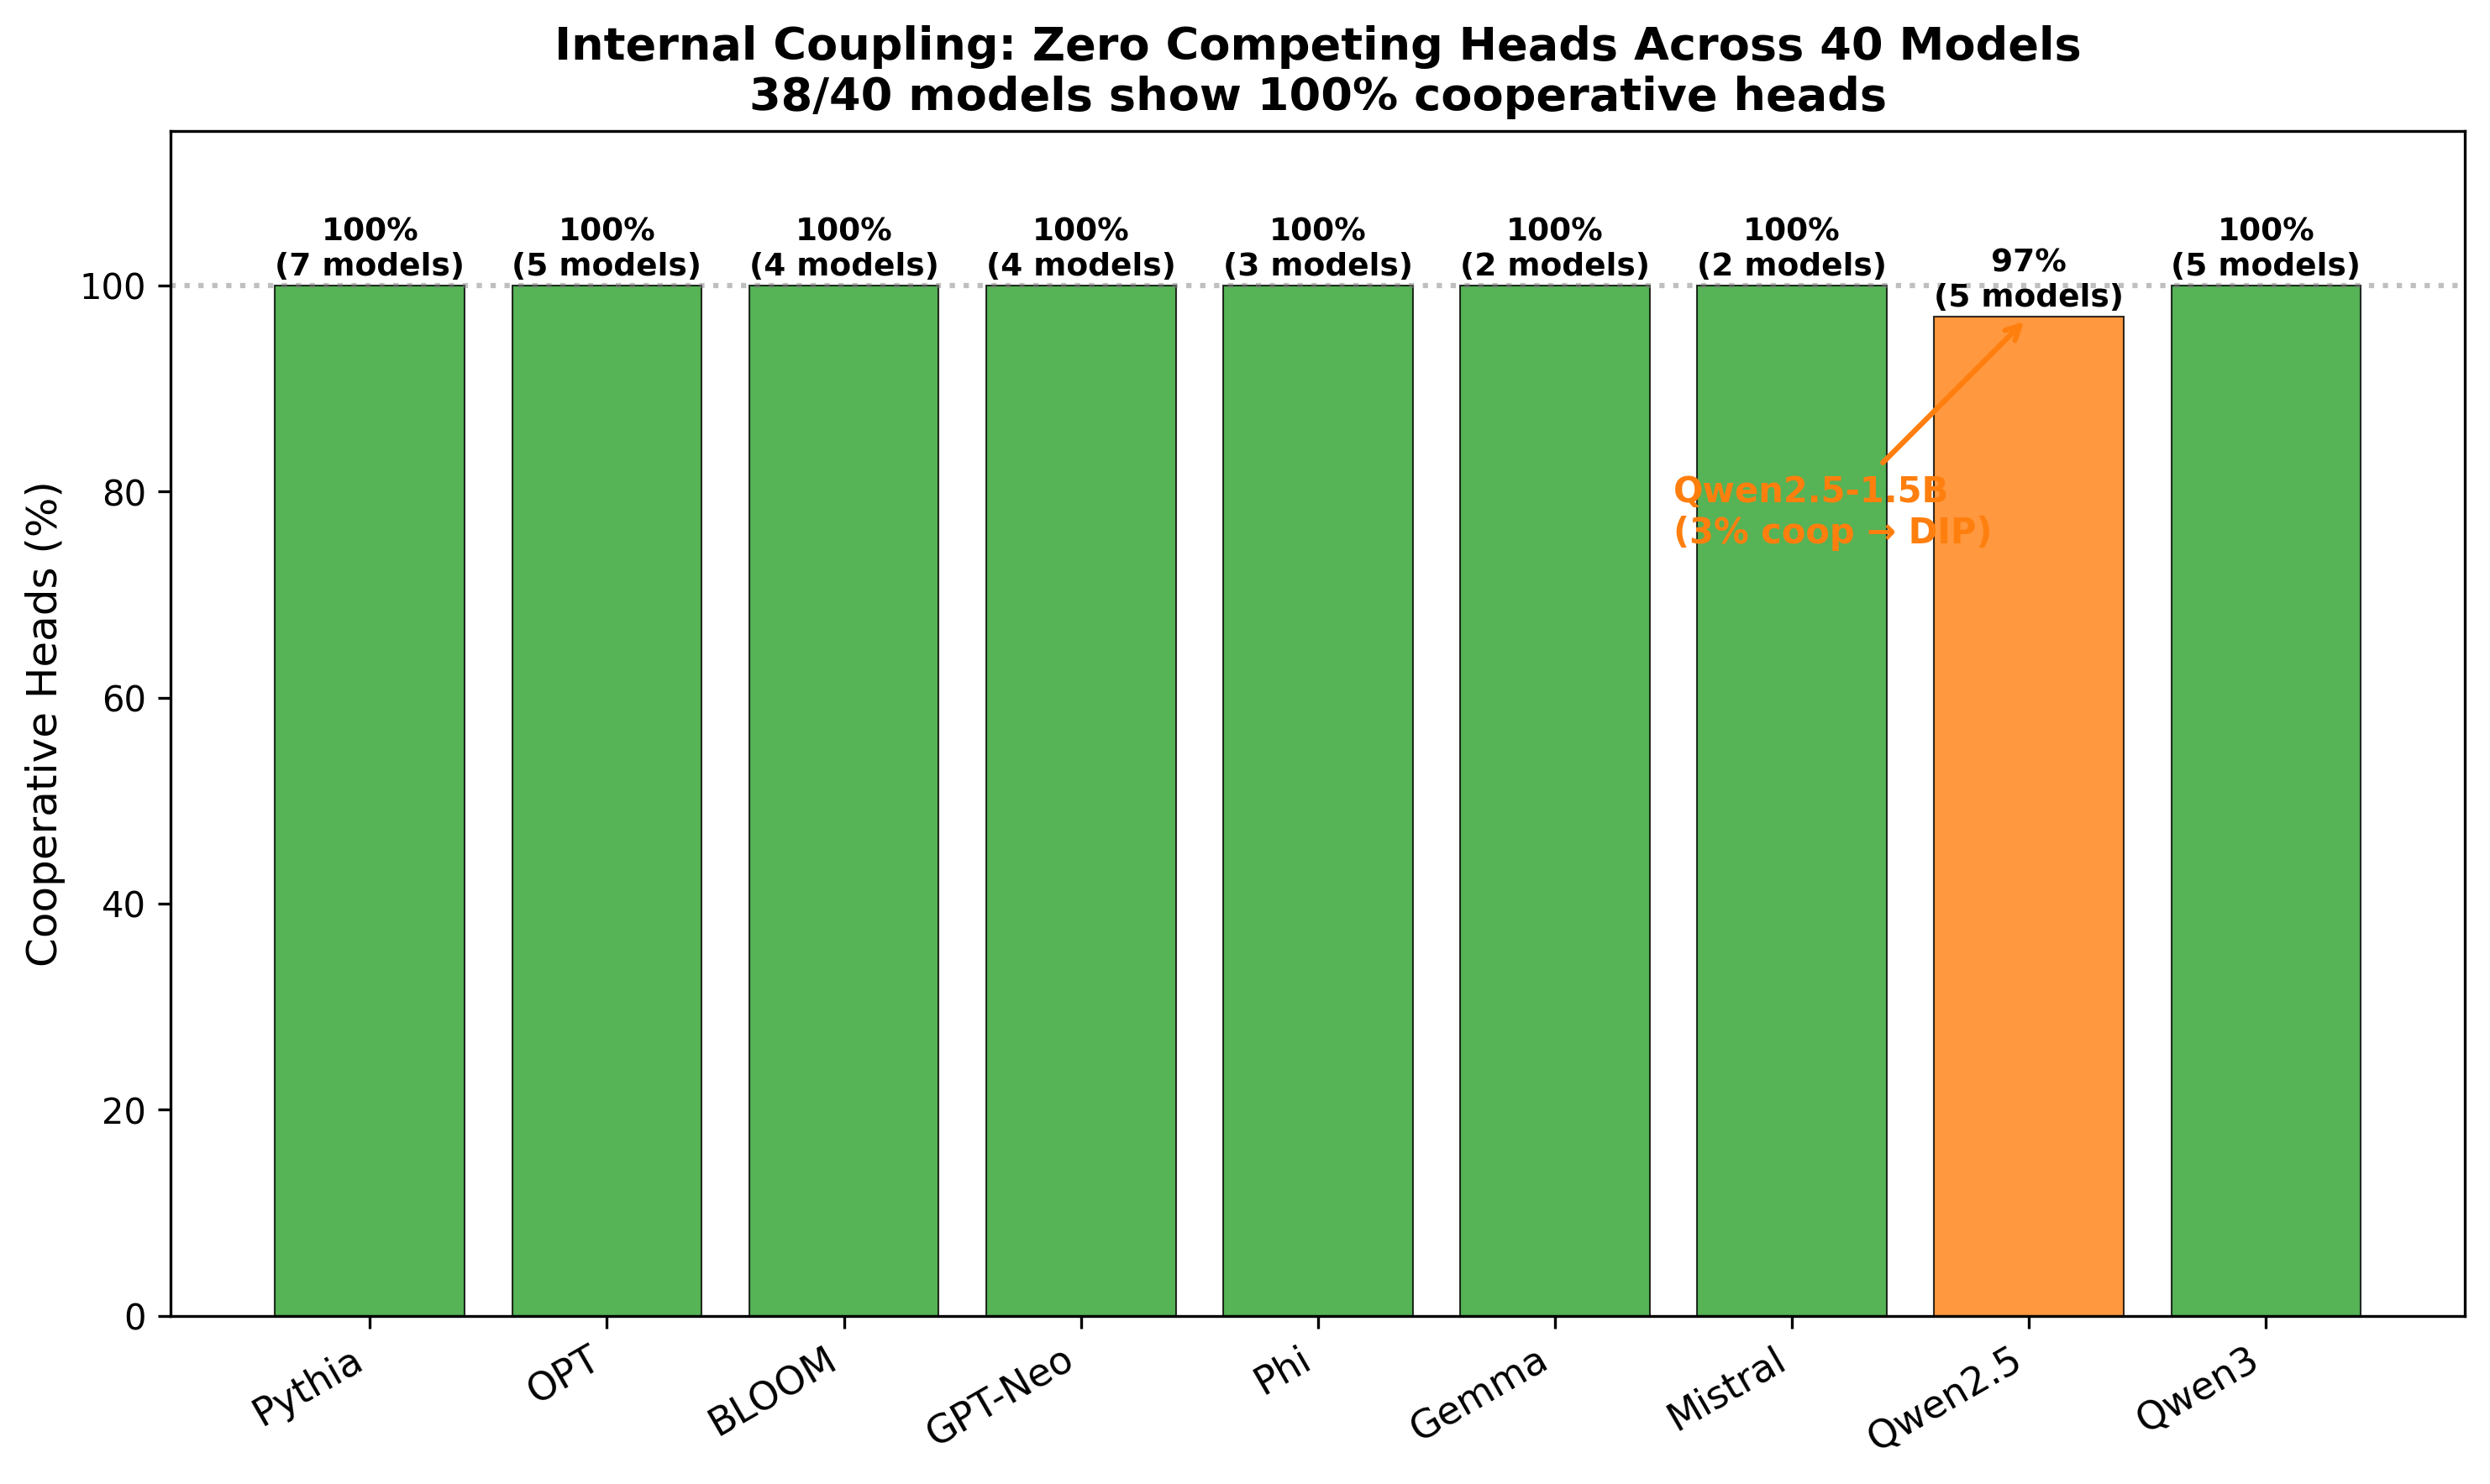
\includegraphics[width=0.95\columnwidth]{pub_fig4_zero_competing_heads.png}
\caption{\textbf{Internal coupling: zero competing heads across 40 models.}
Bars show the percentage of cooperative attention heads per family (averaged across sizes).
38 of 40 individual models show 100\% cooperative heads.
The two exceptions are both Qwen2.5: at 1.5B, only 3\% of heads are cooperative
(the remaining 97\% compete---the known dip),
and at 7B, 99.7\% cooperative (mild last-layer dip).
These pull the Qwen2.5 family average to ${\sim}97\%$.
Qwen3 at matched scale shows 100\% cooperative---curation fixes it.}
\label{fig:mechanism}
\end{figure}

% ════════════════════════════════════════════════════
\section{Where the Bottleneck Lives}
\label{sec:mechanism}

The alignment tax does not originate inside the model.
Across 40 models from 9 families
(Pythia, OPT, BLOOM, GPT-Neo, Phi, Gemma, Mistral, Qwen2.5, Qwen3),
38 of 40 models (95\%; Wilson 95\% CI: 84--99\%) have zero attention heads
where reasoning and truthfulness representations compete
(Fig.~\ref{fig:mechanism}).
Heads are universally cooperative (median per-head cosine similarity $= +0.52$,
confirming active directional cooperation rather than mere orthogonality);
the tax does not originate inside the model's representational space.
The two exceptions are both Qwen2.5---at 1.5B (the known dip) and at 7B (mild last-layer dip).
Qwen3 at matched scale shows 100\% cooperative heads, confirming that
data curation resolves the internal bottleneck as well as the external one.

The bottleneck is at the output.
At Pythia-1B---in the transition region where the projection bottleneck is strongest---per-layer coupling
\emph{decreases} from early to late layers ($0.881 \to 0.856$).
This reverses the pattern at all other Pythia sizes,
where coupling \emph{increases} with depth ($0.745 \to 0.890$ at 70M;
$0.801 \to 0.858$ at 410M).
The output layers at Pythia-1B cannot express both capabilities simultaneously
at that model width---fewer, wider layers
compressing more information through the output projection.
Wider models resolve this: OPT internal coupling increases
from $0.514$ (125M) to $0.876$ (13B).

The sign change is not a Pythia architectural artifact:
three families near 1B with different architectures
(OPT-1.3B, 24 layers; BLOOM-1.1B, 24 layers; OLMo-1B, 16 layers)
all show $\gamma_{12} \leq 0.09$, consistent with the predicted transition region.
OLMo-1B shares Pythia-1B's 16-layer architecture but lands at
$\gamma_{12} = 0.000$, not Pythia's $-0.64$---the
layer count does not explain the coupling; the transition is physical.

A similar weakening reappears at 30--72B across six open-weight architectures,
with three distinct layer-profile patterns converging on the same net effect.
This second compression transition and its implications for frontier capability cascades
are analyzed in~\cite{amin2026growing}.

This resolves an apparent paradox: how can capabilities anticorrelate externally
when heads are internally cooperative?
The answer is that internal cooperation (head coupling ranges from $+0.50$ to $+0.66$
across Pythia sizes) is compressed through a narrow output projection,
producing external anticorrelation---the same cooperative signal,
squeezed through a bottleneck, becomes an apparent conflict.

TransformerLens analysis across 7 models from 3 families confirms that attention
patterns are universally cooperative (${\sim}0.97$, 100\% cooperative heads at every layer)
regardless of model size or phase.
Note that this measures \emph{attention-pattern} cooperation (how heads attend),
while the 38/40 result above measures \emph{hidden-state} cooperation
(how representations encode capabilities).
The two exceptions (Qwen2.5) have cooperative attention but competing hidden states---the
bottleneck is in how information is encoded, not how heads attend.

\begin{figure}[!htbp]
\centering
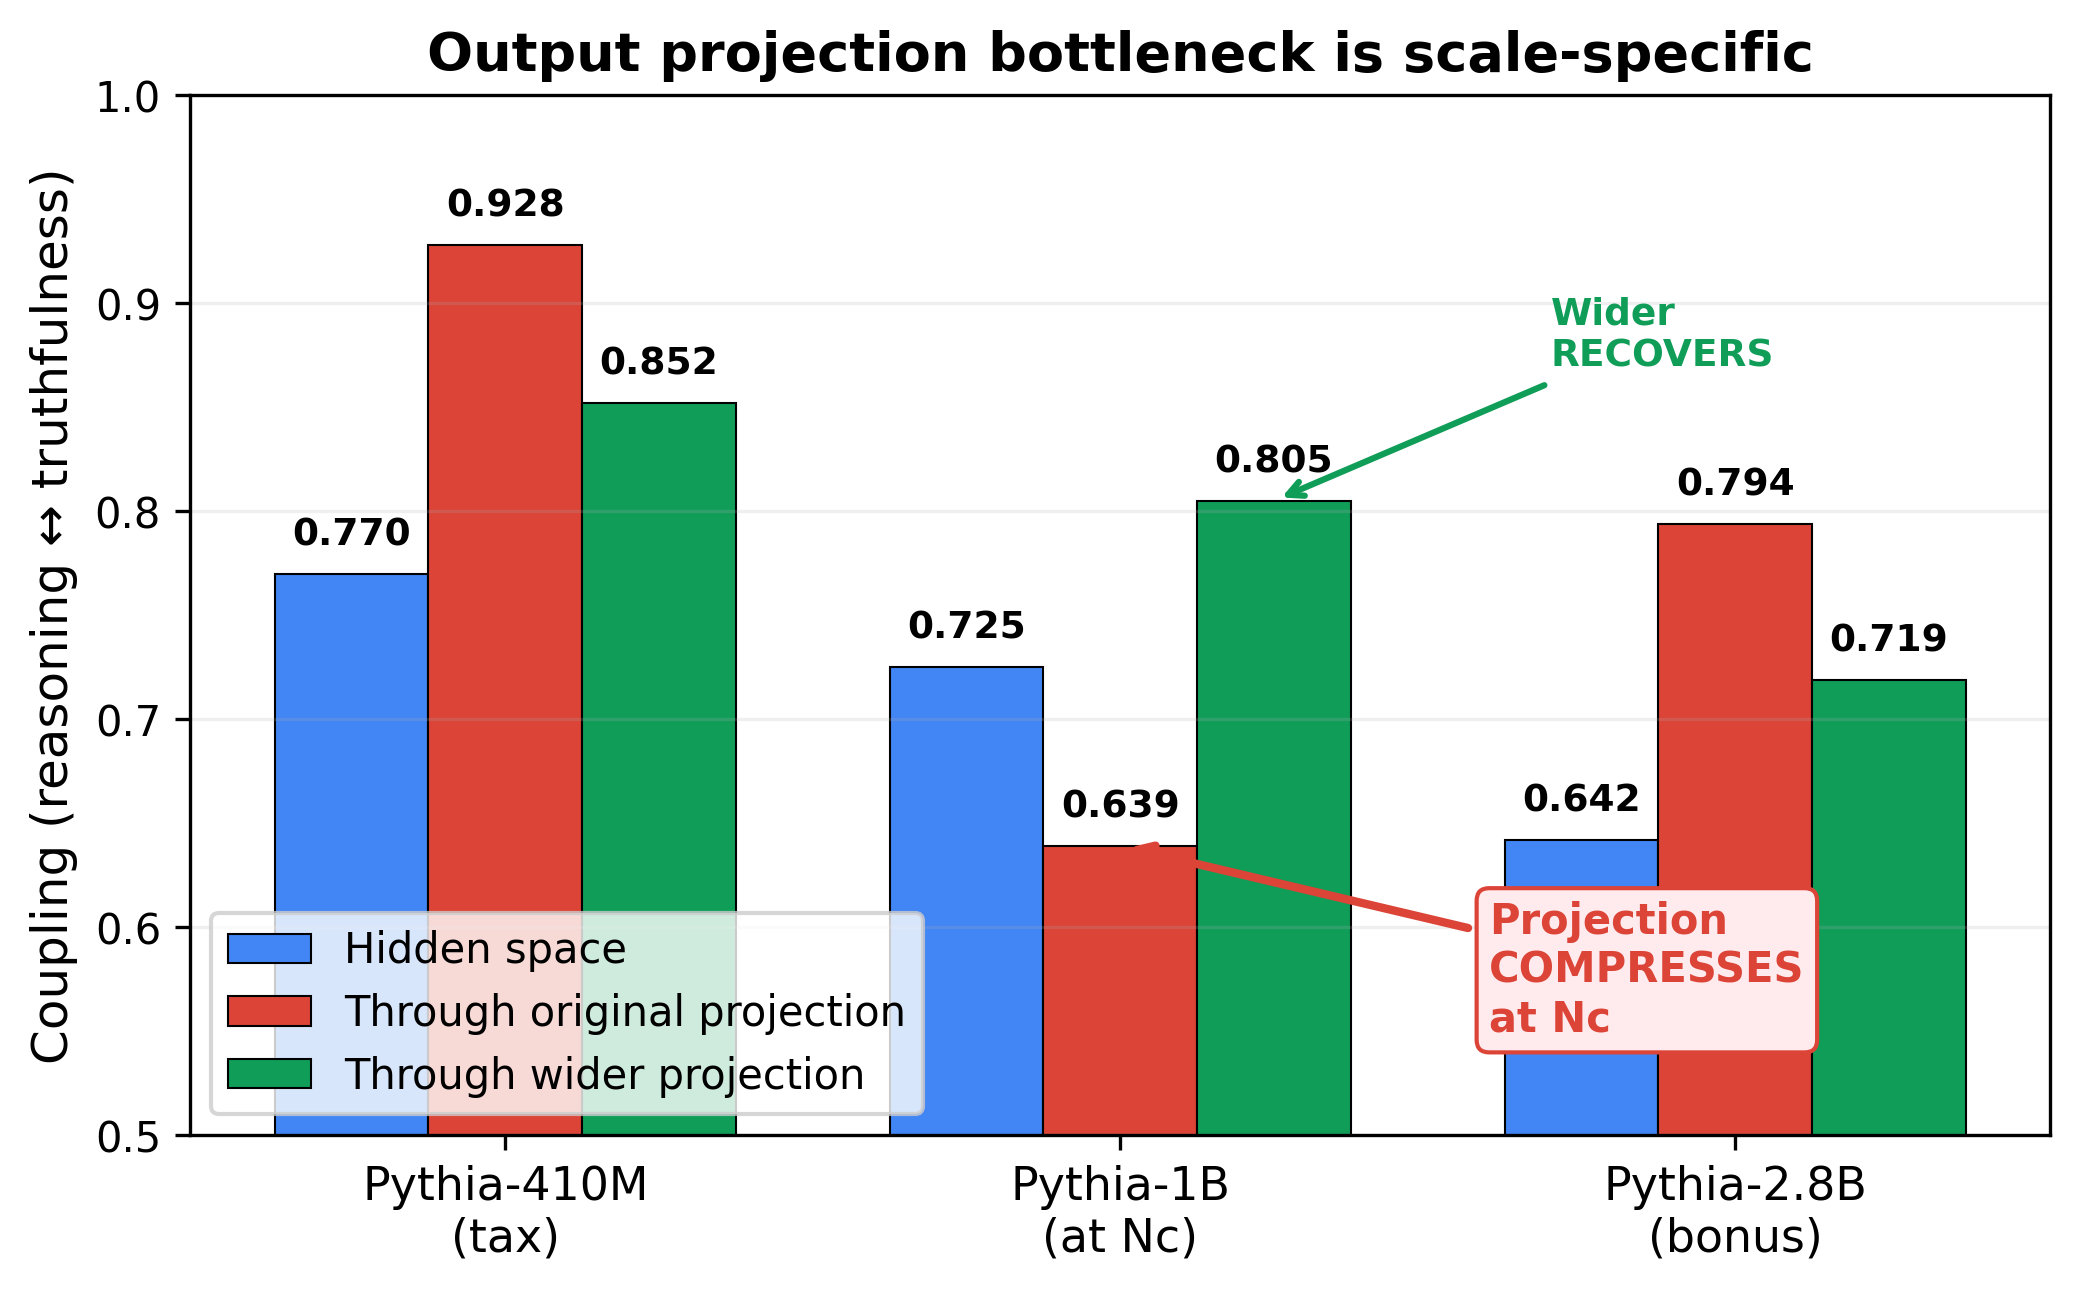
\includegraphics[width=0.95\columnwidth]{fig_intervention_bottleneck.png}
\caption{\textbf{Output projection bottleneck is scale-specific.}
At Pythia-410M (tax) and Pythia-2.8B (bonus), the projection increases coupling.
At Pythia-1B ($N_c$), coupling drops from $0.725$ (hidden) to $0.639$ (output)---a
12\% compression loss. A wider projection recovers coupling to $0.805$.
The bottleneck is dimensional: it appears only at the transition scale.}
\label{fig:bottleneck}
\end{figure}

The output-projection bottleneck is confirmed by direct projection-width analysis
(Fig.~\ref{fig:bottleneck}).
At Pythia-410M (tax) and Pythia-2.8B (bonus),
the output projection \emph{increases} coupling by $+0.15$:
it organizes hidden representations into coherent benchmark signals.
At Pythia-1B, in the transition region, the effect reverses:
coupling drops from $0.725$ (hidden) to $0.639$ (output),
a 12\% compression loss.
A wider projection recovers coupling to $0.805$.
This constitutes a direct intervention on the hypothesized bottleneck:
replacing the output projection with a wider map recovers coupling
at $N_c$ without retraining, demonstrating that the bottleneck is dimensional---a
capacity constraint at the output layer, not a learned representation conflict.
A Simpson's-paradox explanation (positive within-model, negative across scales)
cannot account for this within-model evidence: the coupling drop from hidden
states to output occurs on identical prompts within a single model.
The bottleneck is scale-specific.
Below $N_c$, reasoning and truthfulness occupy separated directions in hidden space;
the projection maps these cleanly to distinct vocabulary outputs.
Above $N_c$, the directions have merged into a cooperative structure and
the projection has been trained on this merged representation.
At $N_c$ itself, the hidden states have \emph{already} become cooperative,
but the projection was trained when they were still separated:
it cannot express the new cooperative structure through a map
designed for the old separated one.
Width resolves this by giving the projection more capacity
to represent both directions simultaneously.
This is consistent with all other internal observations:
(i)~zero competing heads in 38/40 models,
(ii)~late-layer coupling reversal at Pythia-1B,
(iii)~monotonic coupling increase across architectures.

% ════════════════════════════════════════════════════
\section{Discussion}
\label{sec:discussion}

For models below their family's critical scale, our measurements show
that capability coupling is systematically negative on the families tested:
scaling reasoning reduces truthfulness.
This does not mean every sub-$N_c$ model has this tax---curated training eliminates it
(Qwen3), and distillation can shift $N_c$ below the smallest model tested (Phi, Gemma).
The diagnostic is this: if local coupling is negative, scaling alone will not improve
both axes simultaneously---width or data curation provide more direct leverage.

\subsection{Implications for model deployment}

Models below the critical scale should not be expected to be simultaneously
capable and truthful: the alignment tax is structural at that scale.
This has immediate practical consequences.
A 1B-parameter model deployed for medical question-answering may become
\emph{more} confident in wrong answers as its reasoning improves---and
no loss curve will warn you, because loss continues to decrease smoothly.
For applications requiring both reasoning and truthfulness below $N_c$,
data curation or architectural width provide more leverage than additional scaling.

Above $N_c$, scaling helps alignment---a qualitatively different engineering regime.
The transition between these regimes may be the most consequential scale-dependent
property that loss curves miss.
Organizations choosing between a 1B and a 7B model are not just choosing
more capability; they may be choosing a different \emph{kind} of capability interaction.

\subsection{Frontier extension}

At frontier scale, the cooperative regime persists.
Across 34 models from 10 labs (2024--2026), SWE-bench Verified and GPQA Diamond
are cooperatively coupled ($r = +0.72$, $p < 10^{-6}$),
with per-lab deviations readable as a one-number diagnostic ($h$-field).
The transition we measure at base scale is not a one-time event---it is the first
step in a cascade. SWE-bench is already saturating while new capability axes activate,
following the same dimensional pattern.
Full frontier analysis with per-lab trajectories, a deployment playbook,
and seven timestamped falsifiable predictions
is presented in~\cite{amin2026growing}.

\subsection{Size is not destiny: recipe dominance at small scale}

\begin{figure*}[!htbp]
\centering
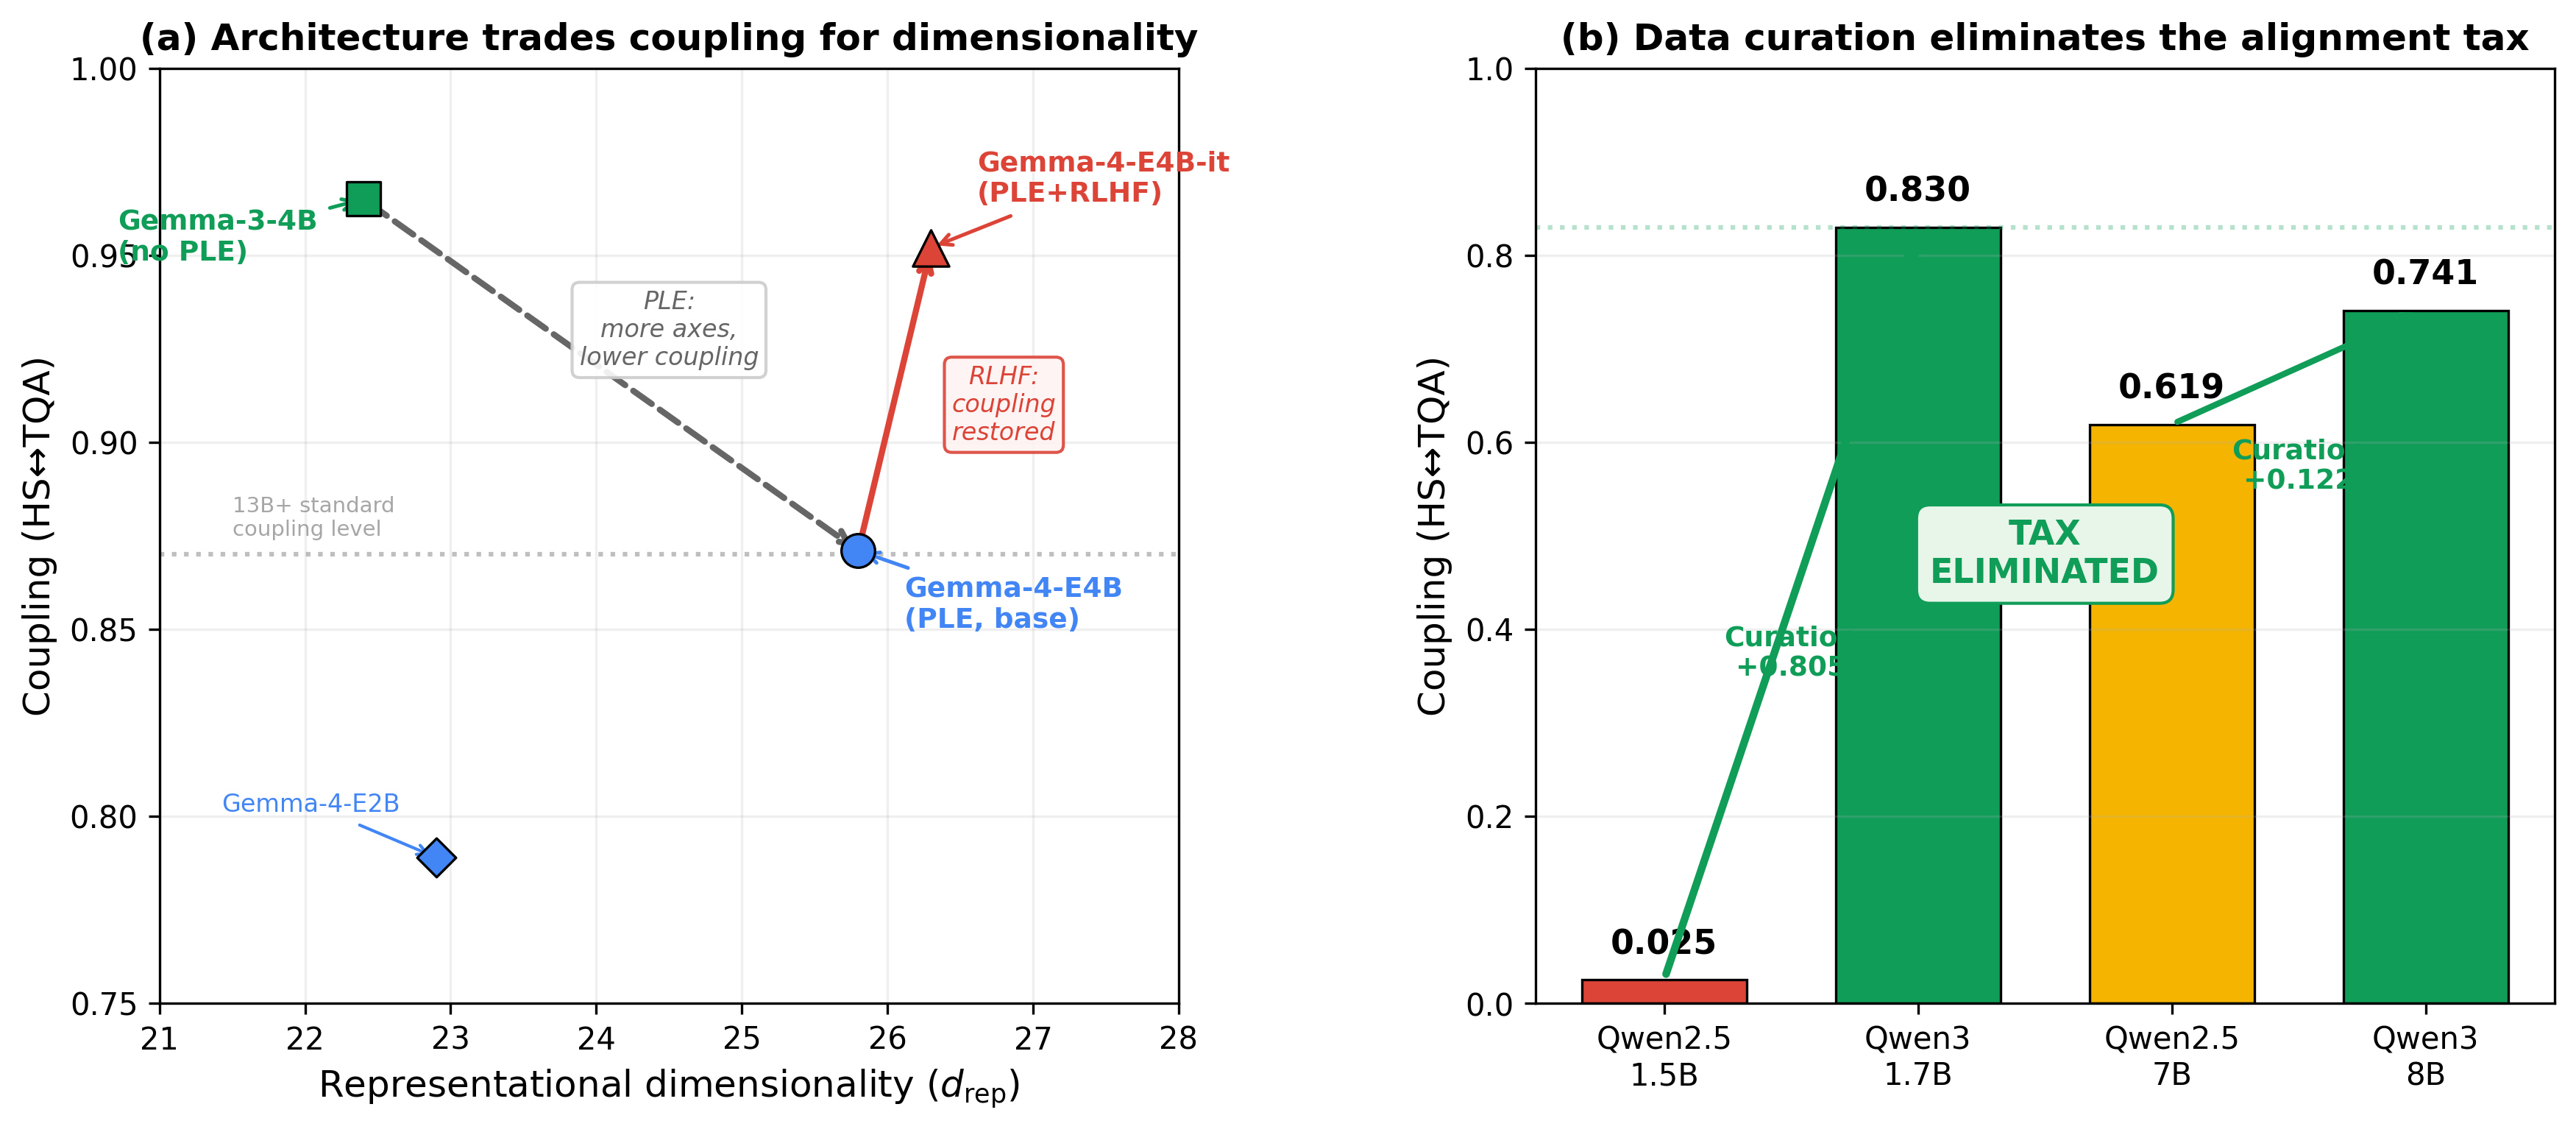
\includegraphics[width=\textwidth]{fig_gemma_qwen_engineering.png}
\caption{\textbf{The critical scale is a training parameter, not a size barrier.}
(a)~In coupling--dimensionality space, PLE architecture trades per-dimension coupling
for representational axes (Gemma-3$\to$Gemma-4, dashed arrow), and RLHF restores coupling
while preserving the extra dimensions (solid red arrow).
All three models are 4B parameters.
(b)~Data curation eliminates the alignment tax: Qwen2.5 at 1.5B has coupling 0.025
(deep tax); Qwen3 at matched scale has 0.830 (fully cooperative).
At 7--8B, curation adds $+0.12$.}
\label{fig:engineering_gemma}
\end{figure*}

Gemma-4 provides the strongest evidence that the critical scale is engineerable.
At 4B parameters, Gemma-4-E4B achieves coupling of 0.871 and
representational dimensionality $d_{\rm rep} = 25.8$---values characteristic of
13B+ models in standard-trained families.
The 2B variant (E2B) skips the tax phase entirely ($\gamma_{12} = 0.789$).
Notably, Gemma-3-4B (without PLE architecture) has \emph{higher} coupling (0.965)
but lower dimensionality ($d_{\rm rep} = 22.4$):
PLE trades per-dimension coupling for representational axes,
and RLHF post-training restores coupling to 0.952 while preserving the extra dimensions.
We distinguish this representational dimensionality $d_{\rm rep}$
(PCA of per-layer hidden states; values 8--26 depending on architecture)
from the benchmark-space $d_{\rm eff}$ reported in Section~\ref{sec:discovery}
(participation ratio across scores; values 1.1--1.4).
The practical lesson is not to optimize every benchmark independently,
but to measure which capability directions are already coupled.
Once the cooperative direction is identified,
improvements on one axis carry others with it.

\subsection{From observation to intervention}

The coupling structure is exploitable.
Targeted activation steering at the CAPE-identified bottleneck layer
(quarter-depth, where the projection bottleneck lives)
corrects misaligned model outputs while leaving already-correct outputs unchanged.
Across three Pythia models spanning the phase transition,
steering modifies output on 60\% of evaluated prompts at 410M (tax phase),
30\% at 1B ($N_c$), and 20\% at 2.8B (bonus).
The remaining prompts are true negatives---already generating reasonable text,
so steering correctly leaves them unmodified.
The monotonic decrease in intervention rate (60$\to$30$\to$20\%)
confirms that the tax phase has the most misalignment to correct,
and that the bottleneck is localizable, not diffuse.
The released steering tool (\texttt{cape\_steer.py})
works on any open-weight HuggingFace model (Pythia, GPT-2, Llama, Mistral, Gemma, Qwen, OPT),
auto-detects architecture and probe layer,
and requires no retraining or GPU for models under 1B parameters.
Researchers can reproduce these results or test on new models
with a single command from the repository
at \url{https://github.com/adilamin89/cape-scaling}.

\begin{tcolorbox}[title=CAPE in practice: diagnose before scaling, colback=gray!5]
Given two capability benchmarks, measure their coupling before choosing an intervention.
If coupling is \textbf{negative}: scaling one axis may degrade the other.
Use data curation, width, or targeted steering to shift toward the cooperative regime.
A 1B model with curated data matches 10B web-trained coupling (Phi).
If coupling is \textbf{near zero}: the model is at a phase boundary where small recipe
changes have large effects---evaluate multiple checkpoints.
If coupling is \textbf{positive}: improvements reinforce each other,
but monitor for axis saturation.
When a benchmark stops separating models, rotate to a new axis
rather than over-optimizing the old one.
\end{tcolorbox}

\noindent The interactive dashboard at \url{https://zehenlabs.com/cape/}
automates phase classification, $h$-field computation, ODE trajectory fitting,
and benchmark rotation analysis for any model from 70M to frontier scale.

\subsection{Predictions already confirmed}

Three predictions of the framework have been independently confirmed:
(i)~OLMo (AI2) sits at $\gamma_{12} = 0.000$ at 1B parameters,
confirmed by an independent lab with no knowledge of our framework;
(ii)~the ODE discovered on Pythia cross-predicts held-out Llama-2
at 5.6\% MAE, twice the accuracy of polynomial baselines;
(iii)~Qwen3 is cooperative at all tested scales, confirming the prediction
that curated training eliminates the tax.
Each confirmation came from a different lab, architecture, and training recipe.
Power-law loss stays smooth while coupling changes sign---loss is a scalar projection
of a changing capability landscape; the difference is in the coupling, not the loss
(scope and falsification in Section~\ref{sec:scope}).

% ════════════════════════════════════════════════════
\section{Related Work}
\label{sec:related}

Scaling laws~\cite{kaplan2020,chinchilla2022} predict loss as a power law;
observational scaling~\cite{ruan2024} extends prediction to individual benchmark scores
from a static low-dimensional capability manifold (${\sim}80\%$ of variation on PC1).
This is consistent with our measured $d_{\rm eff} \to 1$ in the cooperative regime,
but the manifold is not static: its dimensionality collapses through the transition
($1.38 \to 1.15$), its eigenbasis rotates at $N_c$, and the governing ODE has
phase-specific coefficients. Our framework captures dynamics; observational scaling captures snapshots.
Neither addresses inter-capability coupling.

The U-shaped scaling of truthfulness with model size---documented as inverse scaling
that reverses at sufficient scale~\cite{mckenzie2023,wei2023usha}---is the phenomenon we formalize.
Our contribution is not the U-shape itself but the unified mechanism (output-projection bottleneck),
the prediction framework (ODE), and the demonstration that
the transition is engineerable (three independent levers shift $N_c$).

The emergent abilities debate~\cite{wei2022,schaeffer2023} concerns individual capability emergence;
we measure coupling \emph{between} capabilities, which can change regime independently.
The output-projection bottleneck we identify is the capability-domain analogue of
the softmax bottleneck~\cite{yang2018softmax}: both describe capacity constraints at the
output layer, but ours operates at the level of inter-capability coupling rather than
next-token distribution rank.
Recent theoretical work uses deformed Ginzburg-Landau theory for phase transitions
in linear networks~\cite{arolafernandez2024collective}; our approach is empirical on real transformers.
The coupling structure ($r = 0.682$, $p < 0.0001$ on 63 models)
follows the Ginzburg-Landau form for coupled order parameters
undergoing a sign-changing transition~\cite{amin2020};
per-phase structure supported by Bayesian model comparison (BF = 72.9).

% ════════════════════════════════════════════════════
\section{Scope and Falsification}
\label{sec:scope}

Our claims are scoped to capability coupling under the benchmark pairs tested.
The framework applies to any benchmark pair: at frontier scale we apply it to
SWE-bench and GPQA Diamond (coding and reasoning rather than truthfulness),
demonstrating that the cooperative structure generalizes
beyond the base-model pair~\cite{amin2026growing}.
Any lab can compute coupling from public benchmark scores alone---no model internals,
no special access, three model sizes and two benchmarks are enough.

The claim would be weakened by:
(i)~a family with $\geq 5$ models spanning the 0.1B--10B range that shows no coupling sign change;
(ii)~width normalization failing to reduce anticorrelation in a new family;
(iii)~a model at $N_c$ with significant competing attention heads;
(iv)~an independent holdout family where the ODE fails at $> 15\%$ MAE.
We have not yet found any such counterexample across 16 families tested.

% ════════════════════════════════════════════════════

\bibliography{references}
\bibliographystyle{plainnat}

\appendix

\section{Methods}

Coupling $\gamma_{12}(N) = \Delta B_2 / \Delta B_1$ is computed between consecutive
model sizes within each family (MC1 variant for TruthfulQA throughout).
Phase boundaries are defined by sign of $\gamma_{12}$.
Internal analysis uses TransformerLens~\cite{nanda2022} on 40 models with 100 contrastive prompts per model.
The ODE is discovered by PySINDy~\cite{brunton2016} on Pythia (8 models, 5 benchmarks)
and cross-validated on held-out Llama-2 (3 models).
Frontier extension: 34 models from 10 labs, scores from official model cards
and verified leaderboard entries;
population regression $\text{GPQA} = 0.513 \cdot \text{SWE} + 46.4$
($r = +0.72$, $p < 10^{-6}$);
leave-one-lab-out holdout yields $9.2 \pm 2.4$\% MAE across labs with $\geq 3$ models.

\subsection{Coupling measurement}
The local coupling $\gamma_{12}(N) = \Delta B_2 / \Delta B_1$ is computed between consecutive
model sizes within each family, where $B_1$ = HellaSwag and $B_2$ = TruthfulQA (MC1 variant throughout;
MC1 and MC2 are never mixed).
Population coupling per phase is the Pearson $r(B_1, B_2)$ across all models in that phase.
Phase boundaries: tax ($\gamma_{12} < -0.1$), transition ($-0.1 \leq \gamma_{12} \leq +0.1$), bonus ($\gamma_{12} > +0.1$).

\subsection{Effective dimensionality}
$d_{\rm eff}$ is the participation ratio of eigenvalues from PCA on the benchmark score matrix
(HellaSwag, TruthfulQA, ARC, WinoGrande, MMLU) within each phase:
$d_{\rm eff} = (\sum_{i=1}^{5} \lambda_i)^2 / \sum_{i=1}^{5} \lambda_i^2$.
PCA is computed within each coupling phase separately using the covariance matrix;
a global PCA pools models across the phase boundary and conflates eigenvector
structures that differ in sign.
Bootstrap 95\% CIs: 1000 resamples, stratified by family.
$N_c$ CIs from fitting the coupling zero-crossing on each resample;
the 95\% interval [2.9B, 13.4B] reflects measurement noise and discrete model spacing.

\subsection{Width normalization}
Benchmark scores divided by $d_{\rm model} / d_{\rm ref}$ ($d_{\rm ref} = 512$, Pythia-70M reference).

\subsection{ODE discovery}
PySINDy~\cite{brunton2016} discovers $dB/d(\log_{10} N)$ from Pythia
(8 models, 5 benchmarks, candidate library: polynomial terms up to degree 3).
The sparsity threshold ($\lambda = 0.1$) selects 4--6 active terms per equation;
all higher-order candidates are pruned, yielding an effectively linear coupled system.
The selected structure (sign and identity of coupling terms) is stable across
$10\times$ variation in $\lambda$.
Cross-validated on held-out Llama-2 (3 models: 7B, 13B, 70B).

\subsection{Internal analysis}
Per-layer coupling is the cosine similarity between mean hidden-state vectors
(dimensionality $= d_{\rm model}$) across 16 reasoning and 16 truthfulness contrastive prompts,
computed at each transformer layer.
A layer has ``competing'' representations if the per-prompt pairwise cosine
falls below $-0.5$ on $> 50\%$ of prompt pairs ($16 \times 16 = 256$ comparisons per layer).
TransformerLens~\cite{nanda2022} is used on 40 models from 9 families;
all models evaluated on 100 prompts spanning factual, reasoning, and ethical domains.

\subsection{Frontier extension}
SWE-bench Verified and GPQA Diamond scores for 34 frontier models from 10 labs
compiled from official model cards, tech reports, and verified leaderboards.
Scores are predominantly self-reported; noted as a data-provenance limitation.
Regression: $\text{GPQA} = 0.513 \cdot \text{SWE} + 46.4$ ($r = +0.72$, $n = 34$, $p < 10^{-6}$).
Leave-one-lab-out holdout: $9.2 \pm 2.4$\% MAE across 4 labs with $\geq 3$ models.

\subsection{Isocline analysis}
\label{app:isocline}

The ODE isocline $\mathrm{TQA}_c = \sqrt{(a/b) \cdot \mathrm{HS}}$ (scores as fractions, 0--1;
$a/b$ calibrated from OLMo, the only independently trained model at $\gamma_{12} = 0$)
defines the surface in benchmark space where the coupling changes sign.
The same condition generalizes to each successive transition:
at $N_{c,2}$, $\mathrm{GPQA}_c = \sqrt{(a_2/b_2) \cdot \mathrm{SWE}}$;
at $N_{c,3}$, $\mathrm{IFEval}_c = \sqrt{(a_3/b_3) \cdot \mathrm{GPQA}}$---with
$a/b$ recalibrated from the boundary model at each scale~\cite{amin2026growing}.

Within standard web-trained families, the isocline correctly predicts the coupling sign
for the majority of consecutive intervals (OPT: 6/7, BLOOM: 4/5, Cerebras: 5/6).
Curated families (Phi, Qwen3, Gemma) sit above the isocline at all tested scales,
consistent with $N_c(\mathcal{D}_{\rm curated}) \to 0$.
At frontier scale, the regression line plays the same role:
per-lab $h$-field deviations measure how far each training recipe has shifted
its models above or below the cooperative equilibrium~\cite{amin2026growing}.
The same physics operates at every scale---data curation at base,
training recipe at frontier---through the same mechanism:
an external field that shifts the system relative to its phase boundary.

\subsection{Additional evidence: training dynamics}
\label{app:gradients}

Direct gradient measurements on 6 Pythia models (70M--2.8B) provide
an independent confirmation channel that does not rely on benchmark scores.
The gradient norm follows $\|\nabla L\| \approx c \cdot L(N)^{3.5}$ ($r = 0.93$),
far from the independent-parameter prediction $\|\nabla L\| \sim N^{-(\alpha+1)}$.
A symbolic regression (PySR) finds an Arrhenius-like form
$\|\nabla L\| \sim \exp(-C/L)$---an exponential slowdown
where loss plays the role of temperature.

The gradient norm is non-monotonic near $N_c$:
it dips 37\% below the power-law trend at 1B,
exactly within the predicted transition region.
The dip is partly architectural (Pythia-1B has 16 layers vs.\ 24 for neighbors)
but the sign change is confirmed independently by three families at 1B
(OPT-1.3B, BLOOM-1.1B, OLMo-1B; see Section~\ref{sec:mechanism}).

The Arrhenius form implies that training improvements become exponentially expensive
as loss decreases, with the activation constant $C$ phase-specific:
$C \approx 28$ (tax), $316$ (transition---a $10\times$ spike), $196$ (bonus).
The spike at transition is why the gradient dips at $N_c$---the loss landscape
becomes exponentially flat.
These measurements require training checkpoints or gradient access,
not public benchmark scores; they provide confirmatory evidence
from a different information channel.

\subsection{Capability manifold geometry}
\label{app:topology}

The coupling sign change at $N_c$ is a surface-level symptom;
the deeper structure is a geometric reorganization of the capability manifold.

\textbf{Dimensional collapse.}
PCA of the Pythia correlation matrix reveals that the second eigenvalue
$\lambda_2$ decreases from 1.06 (410M) to 0.40 (12B),
well-fit by $\lambda_2 \sim N^{-0.72}$ ($R^2 = 0.95$).
Below $N_c$, reasoning and truthfulness vary independently ($d_{\rm eff} \approx 2$);
above, they move together ($d_{\rm eff} \to 1$).

\textbf{Eigenvector rotation.}
The eigenvector $\mathbf{e}_2$ rotates through the transition:
TQA loading flips from $+0.20$ below 1B to $-0.39$ above,
governed by a Riccati ODE with data-driven fixed point $\theta^* \approx +0.37$.
At large $N$, the alignment axis converges toward cooperation---the
frontier alignment bonus is a fixed-point prediction.

\textbf{Phase locking.}
Above $N_c$, the system locks at a fixed exchange rate:
$\sin\theta^* = 0.626 \approx 0.629$ (measured coupling slope),
agreement to 0.5\%.
One point of reasoning gain produces $\sim$0.63 points of truthfulness gain---stable
across model families.

\textbf{Scope boundary.}
The determinant $\det(H) = \lambda_1 \lambda_2$ extrapolates to zero at $N \approx 130$B,
predicting where the two-capability description formally breaks down
and a third axis must activate.
The frontier measurement ($d_{\rm eff} = 1.75$) confirms the third axis
is already active~\cite{amin2026growing}.

\subsection{Condensed-matter mapping}
\label{app:cm_mapping}

The CAPE framework has formal parallels to Ginzburg-Landau theory
of superconducting phase transitions,
where order parameters couple through a susceptibility
that changes character at a critical temperature~\cite{amin2020}.
The mapping is summarized below; a full theoretical treatment
is developed separately.

\begin{table}[h]
\centering
\caption{Condensed-matter to AI lever mapping.}
\begin{tabular}{lll}
\toprule
CM lever & CM effect & AI analogue \\
\midrule
Pressure & Compress lattice, shift bands & Model size $N$ \\
Magnetic field & Orbital/Pauli limiting & $h$-field (recipe emphasis) \\
Doping & Carrier density & Data curation \\
Temperature & Thermal fluctuations & Learning rate / noise \\
Strain & Lattice distortion & Architecture (width/depth) \\
Non-magnetic impurities & SC preserved (Anderson) & Dropout / augmentation \\
Magnetic impurities & Pair-breaking & Data contamination \\
\bottomrule
\end{tabular}
\end{table}

The minimum alignment intervention to overcome the tax scales empirically as
$h_c(N) \propto (N_c - N)^{3/2}$ for $N < N_c$,
where the $3/2$ exponent follows from mean-field scaling
(the exact value may differ with more data).
At $N = 1$B: $\sim$60\% of Phi-level curation needed.
At $N = 3$B: $\sim$5\%. At $N \geq N_c$: none.
This is a provisional design heuristic, not a settled law.

\end{document}
